\documentclass[output=paper,
modfonts
]{LSP/langsci}
% \bibliography{localbibliography}

% % add all extra packages you need to load to this file 
% \usepackage{todo} %% removed,cna use todonotes instead. % Jason reactivated
% \usepackage{graphicx} % not needed because forest loads tikz, which loads graphicx
\usepackage{tabularx}
\usepackage{amsmath} 
\usepackage{multicol}
\usepackage{lipsum}
\usepackage{longtable}
\usepackage{booktabs}
\usepackage[normalem]{ulem}
%\usepackage{tikz} % not needed because forest loads tikz
\usepackage{phonrule} % for SPE-style phonological rules
\usepackage{pst-all} % loads the main pstricks tools; for arrow diagrams in Hale.tex
%\usepackage{leipzig} % for gloss abbreviations
\usepackage[% for automatic cross-referencing
compress,%
capitalize,% labels are always capitalized in LSP style
noabbrev]% labels are always spelled out in LSP style
{cleveref}

% based on http://tex.stackexchange.com/a/318983/42880 for using gb4e examples with cleveref
\crefname{xnumi}{}{}
\creflabelformat{xnumi}{(#2#1#3)}
\crefrangeformat{xnumi}{(#3#1#4)--(#5#2#6)}
\crefname{xnumii}{}{}
\creflabelformat{xnumii}{(#2#1#3)}
\crefrangeformat{xnumii}{(#3#1#4)--(#5#2#6)}

%\usepackage[notcite,notref]{showkeys} %%removed, not helping CB.
%\usepackage{showidx} %%remove for final compiling - shows index keys at top of page.
 
\usepackage{langsci/styles/langsci-gb4e}  
 \usepackage{pifont}
% % OT tableaux                                                
% \usepackage{pstricks,colortab}  
\usepackage{multirow} % used in OT tableaux
\usepackage{rotating} %needed for angled text%
\usepackage{colortbl} % for cell shading
 
 \usepackage{avm}  
\usepackage[linguistics]{forest} 
\usetikzlibrary{matrix,fit} % for matrix of nodes in Kaisse and Bat-El


\usepackage{hhline}
\newcommand{\cgr}{\cellcolor[gray]{0.8}}
\newcommand{\cn}{\centering}



\newcommand{\reff}[1]{(\ref{#1})}
%\usepackage{newtxtext,newtxmath}


%\usepackage[normalem] {ulem}
\usepackage{qtree}
%\usepackage{natbib}
%\usepackage{tikz}
%\usepackage{gb4e}
\usepackage{phonrule}  
%\bibliographystyle{humannat}



\usepackage{minibox}

%\include{psheader-metr}

\def\bl#1{$_{\textrm{{\footnotesize #1}}}$}
%% add all extra packages you need to load to this file 
\usepackage{todo}
\usepackage{graphicx}
\usepackage{tabularx}
\usepackage{amsmath} 
\usepackage{multicol}
\usepackage{lipsum}
\usepackage{longtable,booktabs}

\usepackage{graphicx}
\usepackage{amsmath}
\usepackage{arydshln}  %allows dashed lines in tables
\usepackage{amssymb}
%\usepackage{tipa} % commented out by Jason Zentz to allow compilation
\usepackage{epstopdf}
\usepackage{qtree}
\usepackage{tree-dvips}
\usepackage{pict2e}
 \usepackage{float}
 \usepackage{textcomp}
 \usepackage{multicol}
\usepackage{datetime}
\usepackage[normalem]{ulem}

%\renewcommand{\dotuline}{\bgroup \markoverwith{\lower .4ex\hbox{.}}\ULon} % commented out by Jason Zentz to allow compilation
\DeclareGraphicsRule{.tif}{png}{.png}{`convert #1 `dirname #1`/`basename #1 .tif`.png}
%%%%%%%%%%%%%%%%%%%%%%%%%%%%%%%%%%%%%%%%%%%%%%%%%%%%
%%%                                              %%%
%%%           Examples                           %%%
%%%                                              %%%
%%%%%%%%%%%%%%%%%%%%%%%%%%%%%%%%%%%%%%%%%%%%%%%%%%%%
% remove the percentage signs in the following lines
% if your book makes use of linguistic examples
\usepackage{LSP/lsp-styles/lsp-gb4e} 
%% to add additional information to the right of examples, uncomment the following line
% \usepackage{jambox}
%% if you want the source line of examples to be in italics, uncomment the following line
% \def\exfont{\it}

%%%%%%%%%%%%%%%%%%%%%%%%%%%%%%%%%%%%%%%%%%%%%%%%%%%%
%%%                                              %%%
%%%      Optimality Theory                       %%%
%%%                                              %%%
%%%%%%%%%%%%%%%%%%%%%%%%%%%%%%%%%%%%%%%%%%%%%%%%%%%%
% If you are using OT, uncomment the following lines      
% % OT pointing hand
% \usepackage{pifont}
% \newcommand{\hand}{\ding{43}}
% % OT tableaux                                                
% \usepackage{pstricks,colortab}    

%%%%%%%%%%%%%%%%%%%%%%%%%%%%%%%%%%%%%%%%%%%%%%%%%%%%
%%%                                              %%%
%%%       Attribute Value Matrices               %%%
%%%                                              %%%
%%%%%%%%%%%%%%%%%%%%%%%%%%%%%%%%%%%%%%%%%%%%%%%%%%%%
%If you are using Attribute-Value-Matrices, uncomment the following lines 
% \usepackage{lsp-avm}
% \usepackage{avm}
% \avmfont{\sc} 
% \avmvalfont{\it} 
% % command to fontify the type values of an avm 
% \newcommand{\tpv}[1]{{\avmjvalfont #1}} 
% % command to fontify the type of an avm and avmspan it
% \newcommand{\tp}[1]{\avmspan{\tpv{#1}}}

%%%%%%%%%%%%%%%%%%%%%%%%%%%%%%%%%%%%%%%%%%%%%%%%%%%%
%%%                                              %%%
%%%     Discourse Representation Structures      %%%
%%%                                              %%%
%%%%%%%%%%%%%%%%%%%%%%%%%%%%%%%%%%%%%%%%%%%%%%%%%%%%
% DRS package by Alexis Dimitriadis
% \usepackage{drs}

%%%%%%%%%%%%%%%%%%%%%%%%%%%%%%%%%%%%%%%%%%%%%%%%%%%%
%%%                                              %%%
%%%            Chinese Japanese Korean           %%%
%%%                                              %%%
%%%%%%%%%%%%%%%%%%%%%%%%%%%%%%%%%%%%%%%%%%%%%%%%%%%%

% For Chinese characters, uncomment the following lines
% \usepackage[indentfirst=false]{xeCJK}
% \setCJKmainfont{SimSun}

%%%%%%%%%%%%%%%%%%%%%%%%%%%%%%%%%%%%%%%%%%%%%%%%%%%%
%%%                                              %%%
%%%               Arabic / Persian               %%%
%%%                                              %%%
%%%%%%%%%%%%%%%%%%%%%%%%%%%%%%%%%%%%%%%%%%%%%%%%%%%%

% for bidirectional text and support for Arabic/Persian, uncomment the following lines
%% \usepackage{fontspec}
% \newfontfamily\Parsifont[Script=Arabic]{XB Niloofar}
% %\usepackage{bidi}
% \usepackage{lsp-bidi}
% \newcommand{\PRL}[1]{\RL{\Parsifont #1}}
% %\TeXXeTOff
 

%%%%%%%%%%%%%%%%%%%%%%%%%%%%%%%%%%%%%%%%%%%%%%%%%%%%
%%%                                              %%%
%%%          Trees                               %%%
%%%                                              %%%
%%%%%%%%%%%%%%%%%%%%%%%%%%%%%%%%%%%%%%%%%%%%%%%%%%%%

% For trees, uncomment the following lines
% \usepackage{tikz-qtree}
% % has strange side effects
% %\tikzset{every tree node/.style={align=left, anchor=north}}
% \tikzset{every roof node/.append style={inner sep=0.1pt,text height=2ex,text depth=0.3ex}}

% %add all your local new commands to this file

\newcommand{\form}[1]{\mbox{\emph{#1}}}
\newcommand{\uf}[1]{\mbox{/#1/}}

% borrowed from expex and converted from plan tex to latex
\newcommand{\judge}[1]{{\upshape #1\hspace{0.1em}}}
\newcommand{\ljudge}[1]{\makebox[0pt][r]{\judge{#1}}}

\newcommand\tikzmark[1]{\tikz[remember picture, baseline=(#1.base)] \node[anchor=base,inner sep=0pt, outer sep=0pt] (#1) {#1};} % for adding decorations, arrows, lines, etc. to text
\newcommand\tikzmarknamed[2]{\tikz[remember picture, baseline=(#1.base)] \node[anchor=base,inner sep=0pt, outer sep=0pt] (#1) {#2};} % for adding decorations, arrows, lines, etc. to text
\newcommand\tikzmarkfullnamed[2]{\tikz[remember picture, baseline=(#1.base)] \node[anchor=base,inner sep=0pt, outer sep=0pt] (#1) {\vphantom{X}#2};} % for adding decorations, arrows, lines, etc. to text; this one works best for decorations above a line of text because it adds in the heigh of a capital letter and takes two arguments - one for the node name and one for the printed text

\newcommand{\sub}[1]{$_{\text{#1}}$} % for non-math subscripts
\newcommand{\subit}[1]{\sub{\textit{#1}}} % for italics non-math subscripts
\newcommand{\1}{\rlap{$'$}\xspace} % for the prime in X' (the \rlap command allows the prime to be ignored for horizontal spacing in trees, and the \xspace command allows you to use this in normal text without adding \ afterwards). This isn't crucial, but it helps the formatting to look a little better.

% Aissen:
\newcommand\tikzmarkfull[1]{\tikz[remember picture, baseline=(#1.base)] \node[anchor=base,inner sep=0pt, outer sep=0pt] (#1) {\vphantom{X}#1};} % for adding decorations, arrows, lines, etc. to text; this one works best for decorations above a line of text because it adds in the heigh of a capital letter and takes one argument that serves as the name and the printed text
\newcommand{\bridgeover}[2]{% for a line that creates a bridge over text, connecting two nodes
	\begin{tikzpicture}[remember picture,overlay]
	\draw[thick,shorten >=3pt,shorten <=3pt] (#1.north) |- +(0ex,2.5ex) -| (#2.north);
	\end{tikzpicture}
}
\newcommand{\bridgeoverht}[3]{% for a line that creates a bridge over text, connecting two nodes and specifing the height of the bridge
	\begin{tikzpicture}[remember picture,overlay]
	\draw[thick,shorten >=3pt,shorten <=3pt] (#2.north) |- +(0ex,#1) -| (#3.north);
	\end{tikzpicture}
}
\newcommand{\bridgeoverex}{\vspace*{3ex}} % place before an example that has a \bridgeover so that there is enough vertical space for it

% Chung:
\newcommand{\lefttabular}[1]{\begin{tabular}{p{0.5in}}#1\end{tabular}}

% Kaisse:
\newcommand{\mgmorph}[1]{|(#1)| {#1}}
\newcommand{\mgone}[2][$\times$]{\node at (#2.base) [above=2ex] (1#2) {\vphantom{X}#1};}
\newcommand{\mgtwo}[2][$\times$]{\mgone{#2} \node at (#2.base) [above=4.5ex] (2#2) {\vphantom{X}#1};}
\newcommand{\mgthree}[2][$\times$]{\mgtwo{#2} \node at (#2.base) [above=7ex] (3#2) {\vphantom{X}#1};}
\newcommand{\mgftl}[1]{\node at (1#1) [left] {(};}
\newcommand{\mgftr}[1]{\node at (1#1) [right] {)};}
\newcommand{\mgfoot}[2]{\mgftl{#1}\mgftr{#2}}
\newcommand{\mgldelim}[2]{\node at (#2.west) [left,inner sep = 0pt, outer sep = 0pt] {#1};}
\newcommand{\mgrdelim}[2]{\node at (#2.east) [right,inner sep = 0pt, outer sep = 0pt] {#1};}

\newcommand{\squish}{\hspace*{-3pt}}

% Kavitskaya:
\newcommand{\assoc}[2]{\draw (#1.south) -- (#2.north);}
\newcolumntype{L}{>{\raggedright\arraybackslash}X}

% Lepic & Padden:
\newcommand{\fitpic}[1]{\resizebox{\hsize}{!}{\includegraphics{#1}}} % from http://tex.stackexchange.com/a/148965/42880
\newcommand{\signpic}[1]{\includegraphics[width=1.36in]{#1}}
\newcolumntype{C}{>{\centering\arraybackslash}X}

% Spencer:

\newcommand{\textex}[1]{\textit{#1}\xspace}
\newcommand{\lxm}[1]{\textsc{#1}\xspace}

% Thrainsson:

\renewcommand{\textasciitilde}{\char`~} % for use with TTF/OTF fonts (see comments on http://tex.stackexchange.com/a/317/42880)
\newcommand{\tikzarrow}[2]{% for an arrow connecting two nodes
\begin{tikzpicture}[remember picture,overlay]
\draw[thick,shorten >=3pt,shorten <=3pt,->,>=stealth] (#1) -- (#2);
\end{tikzpicture}
}

\newlength{\padding}
\setlength{\padding}{0.5em}
\newcommand{\lesspadding}{\hspace*{-\padding}}
\newcommand{\feat}[1]{\lesspadding#1\lesspadding}

% Hammond

\usepackage[]{graphicx}\usepackage[]{xcolor}
%% maxwidth is the original width if it is less than linewidth
%% otherwise use linewidth (to make sure the graphics do not exceed the margin)
\makeatletter
\def\maxwidth{ %
  \ifdim\Gin@nat@width>\linewidth
    \linewidth
  \else
    \Gin@nat@width
  \fi
}
\makeatother

\definecolor{fgcolor}{rgb}{0.345, 0.345, 0.345}
\newcommand{\hlnum}[1]{\textcolor[rgb]{0.686,0.059,0.569}{#1}}%
\newcommand{\hlstr}[1]{\textcolor[rgb]{0.192,0.494,0.8}{#1}}%
\newcommand{\hlcom}[1]{\textcolor[rgb]{0.678,0.584,0.686}{\textit{#1}}}%
\newcommand{\hlopt}[1]{\textcolor[rgb]{0,0,0}{#1}}%
\newcommand{\hlstd}[1]{\textcolor[rgb]{0.345,0.345,0.345}{#1}}%
\newcommand{\hlkwa}[1]{\textcolor[rgb]{0.161,0.373,0.58}{\textbf{#1}}}%
\newcommand{\hlkwb}[1]{\textcolor[rgb]{0.69,0.353,0.396}{#1}}%
\newcommand{\hlkwc}[1]{\textcolor[rgb]{0.333,0.667,0.333}{#1}}%
\newcommand{\hlkwd}[1]{\textcolor[rgb]{0.737,0.353,0.396}{\textbf{#1}}}%
\let\hlipl\hlkwb

\usepackage{framed}
\makeatletter
\newenvironment{kframe}{%
 \def\at@end@of@kframe{}%
 \ifinner\ifhmode%
  \def\at@end@of@kframe{\end{minipage}}%
  \begin{minipage}{\columnwidth}%
 \fi\fi%
 \def\FrameCommand##1{\hskip\@totalleftmargin \hskip-\fboxsep
 \colorbox{shadecolor}{##1}\hskip-\fboxsep
     % There is no \\@totalrightmargin, so:
     \hskip-\linewidth \hskip-\@totalleftmargin \hskip\columnwidth}%
 \MakeFramed {\advance\hsize-\width
   \@totalleftmargin\z@ \linewidth\hsize
   \@setminipage}}%
 {\par\unskip\endMakeFramed%
 \at@end@of@kframe}
\makeatother

\definecolor{shadecolor}{rgb}{.97, .97, .97}
\definecolor{messagecolor}{rgb}{0, 0, 0}
\definecolor{warningcolor}{rgb}{1, 0, 1}
\definecolor{errorcolor}{rgb}{1, 0, 0}
\newenvironment{knitrout}{}{} % an empty environment to be redefined in TeX

\usepackage{alltt}

%revised version started: 12/17/16

%NEEDS: allbib.bib - already added to the master bibliography file.
%cited references only: bibexport -o mhTMP.bib main1-blx.aux
%PLUS sramh-img*, sramh.tex

%added stuff
\newcommand{\add}[1]{\textcolor{blue}{#1}}
%deleted stuff
\newcommand{\del}[1]{\textcolor{red}{(removed: #1)}}
%uncomment these to turn off colors
\renewcommand{\add}[1]{#1}
\renewcommand{\del}[1]{}

%shortcuts
\newcommand{\w}{\ili{Welsh}}
\newcommand{\e}{\ili{English}}
\newcommand{\io}{Input Optimization}




 \newcommand{\hand}{\ding{43}}
% \newcommand{\rot}[1]{\begin{rotate}{90}#1\end{rotate}} %shortcut for angled text%  
% \newcommand{\rotcon}[1]{\raisebox{-5ex}{\hspace*{1ex}\rot{\hspace*{1ex}#1}}}

%% add all extra packages you need to load to this file 
% \usepackage{todo} %% removed,cna use todonotes instead. % Jason reactivated
% \usepackage{graphicx} % not needed because forest loads tikz, which loads graphicx
\usepackage{tabularx}
\usepackage{amsmath} 
\usepackage{multicol}
\usepackage{lipsum}
\usepackage{longtable}
\usepackage{booktabs}
\usepackage[normalem]{ulem}
%\usepackage{tikz} % not needed because forest loads tikz
\usepackage{phonrule} % for SPE-style phonological rules
\usepackage{pst-all} % loads the main pstricks tools; for arrow diagrams in Hale.tex
%\usepackage{leipzig} % for gloss abbreviations
\usepackage[% for automatic cross-referencing
compress,%
capitalize,% labels are always capitalized in LSP style
noabbrev]% labels are always spelled out in LSP style
{cleveref}

% based on http://tex.stackexchange.com/a/318983/42880 for using gb4e examples with cleveref
\crefname{xnumi}{}{}
\creflabelformat{xnumi}{(#2#1#3)}
\crefrangeformat{xnumi}{(#3#1#4)--(#5#2#6)}
\crefname{xnumii}{}{}
\creflabelformat{xnumii}{(#2#1#3)}
\crefrangeformat{xnumii}{(#3#1#4)--(#5#2#6)}

%\usepackage[notcite,notref]{showkeys} %%removed, not helping CB.
%\usepackage{showidx} %%remove for final compiling - shows index keys at top of page.
 
\usepackage{langsci/styles/langsci-gb4e}  
 \usepackage{pifont}
% % OT tableaux                                                
% \usepackage{pstricks,colortab}  
\usepackage{multirow} % used in OT tableaux
\usepackage{rotating} %needed for angled text%
\usepackage{colortbl} % for cell shading
 
 \usepackage{avm}  
\usepackage[linguistics]{forest} 
\usetikzlibrary{matrix,fit} % for matrix of nodes in Kaisse and Bat-El


\usepackage{hhline}
\newcommand{\cgr}{\cellcolor[gray]{0.8}}
\newcommand{\cn}{\centering}



\newcommand{\reff}[1]{(\ref{#1})}
%\usepackage{newtxtext,newtxmath}


%\usepackage[normalem] {ulem}
\usepackage{qtree}
%\usepackage{natbib}
%\usepackage{tikz}
%\usepackage{gb4e}
\usepackage{phonrule}  
%\bibliographystyle{humannat}



\usepackage{minibox}

%\include{psheader-metr}

\def\bl#1{$_{\textrm{{\footnotesize #1}}}$}
\usepackage{arydshln}
\usepackage{rotating}

%%add all your local new commands to this file

\newcommand{\form}[1]{\mbox{\emph{#1}}}
\newcommand{\uf}[1]{\mbox{/#1/}}

% borrowed from expex and converted from plan tex to latex
\newcommand{\judge}[1]{{\upshape #1\hspace{0.1em}}}
\newcommand{\ljudge}[1]{\makebox[0pt][r]{\judge{#1}}}

\newcommand\tikzmark[1]{\tikz[remember picture, baseline=(#1.base)] \node[anchor=base,inner sep=0pt, outer sep=0pt] (#1) {#1};} % for adding decorations, arrows, lines, etc. to text
\newcommand\tikzmarknamed[2]{\tikz[remember picture, baseline=(#1.base)] \node[anchor=base,inner sep=0pt, outer sep=0pt] (#1) {#2};} % for adding decorations, arrows, lines, etc. to text
\newcommand\tikzmarkfullnamed[2]{\tikz[remember picture, baseline=(#1.base)] \node[anchor=base,inner sep=0pt, outer sep=0pt] (#1) {\vphantom{X}#2};} % for adding decorations, arrows, lines, etc. to text; this one works best for decorations above a line of text because it adds in the heigh of a capital letter and takes two arguments - one for the node name and one for the printed text

\newcommand{\sub}[1]{$_{\text{#1}}$} % for non-math subscripts
\newcommand{\subit}[1]{\sub{\textit{#1}}} % for italics non-math subscripts
\newcommand{\1}{\rlap{$'$}\xspace} % for the prime in X' (the \rlap command allows the prime to be ignored for horizontal spacing in trees, and the \xspace command allows you to use this in normal text without adding \ afterwards). This isn't crucial, but it helps the formatting to look a little better.

% Aissen:
\newcommand\tikzmarkfull[1]{\tikz[remember picture, baseline=(#1.base)] \node[anchor=base,inner sep=0pt, outer sep=0pt] (#1) {\vphantom{X}#1};} % for adding decorations, arrows, lines, etc. to text; this one works best for decorations above a line of text because it adds in the heigh of a capital letter and takes one argument that serves as the name and the printed text
\newcommand{\bridgeover}[2]{% for a line that creates a bridge over text, connecting two nodes
	\begin{tikzpicture}[remember picture,overlay]
	\draw[thick,shorten >=3pt,shorten <=3pt] (#1.north) |- +(0ex,2.5ex) -| (#2.north);
	\end{tikzpicture}
}
\newcommand{\bridgeoverht}[3]{% for a line that creates a bridge over text, connecting two nodes and specifing the height of the bridge
	\begin{tikzpicture}[remember picture,overlay]
	\draw[thick,shorten >=3pt,shorten <=3pt] (#2.north) |- +(0ex,#1) -| (#3.north);
	\end{tikzpicture}
}
\newcommand{\bridgeoverex}{\vspace*{3ex}} % place before an example that has a \bridgeover so that there is enough vertical space for it

% Chung:
\newcommand{\lefttabular}[1]{\begin{tabular}{p{0.5in}}#1\end{tabular}}

% Kaisse:
\newcommand{\mgmorph}[1]{|(#1)| {#1}}
\newcommand{\mgone}[2][$\times$]{\node at (#2.base) [above=2ex] (1#2) {\vphantom{X}#1};}
\newcommand{\mgtwo}[2][$\times$]{\mgone{#2} \node at (#2.base) [above=4.5ex] (2#2) {\vphantom{X}#1};}
\newcommand{\mgthree}[2][$\times$]{\mgtwo{#2} \node at (#2.base) [above=7ex] (3#2) {\vphantom{X}#1};}
\newcommand{\mgftl}[1]{\node at (1#1) [left] {(};}
\newcommand{\mgftr}[1]{\node at (1#1) [right] {)};}
\newcommand{\mgfoot}[2]{\mgftl{#1}\mgftr{#2}}
\newcommand{\mgldelim}[2]{\node at (#2.west) [left,inner sep = 0pt, outer sep = 0pt] {#1};}
\newcommand{\mgrdelim}[2]{\node at (#2.east) [right,inner sep = 0pt, outer sep = 0pt] {#1};}

\newcommand{\squish}{\hspace*{-3pt}}

% Kavitskaya:
\newcommand{\assoc}[2]{\draw (#1.south) -- (#2.north);}
\newcolumntype{L}{>{\raggedright\arraybackslash}X}

% Lepic & Padden:
\newcommand{\fitpic}[1]{\resizebox{\hsize}{!}{\includegraphics{#1}}} % from http://tex.stackexchange.com/a/148965/42880
\newcommand{\signpic}[1]{\includegraphics[width=1.36in]{#1}}
\newcolumntype{C}{>{\centering\arraybackslash}X}

% Spencer:

\newcommand{\textex}[1]{\textit{#1}\xspace}
\newcommand{\lxm}[1]{\textsc{#1}\xspace}

% Thrainsson:

\renewcommand{\textasciitilde}{\char`~} % for use with TTF/OTF fonts (see comments on http://tex.stackexchange.com/a/317/42880)
\newcommand{\tikzarrow}[2]{% for an arrow connecting two nodes
\begin{tikzpicture}[remember picture,overlay]
\draw[thick,shorten >=3pt,shorten <=3pt,->,>=stealth] (#1) -- (#2);
\end{tikzpicture}
}

\newlength{\padding}
\setlength{\padding}{0.5em}
\newcommand{\lesspadding}{\hspace*{-\padding}}
\newcommand{\feat}[1]{\lesspadding#1\lesspadding}

% Hammond

\usepackage[]{graphicx}\usepackage[]{xcolor}
%% maxwidth is the original width if it is less than linewidth
%% otherwise use linewidth (to make sure the graphics do not exceed the margin)
\makeatletter
\def\maxwidth{ %
  \ifdim\Gin@nat@width>\linewidth
    \linewidth
  \else
    \Gin@nat@width
  \fi
}
\makeatother

\definecolor{fgcolor}{rgb}{0.345, 0.345, 0.345}
\newcommand{\hlnum}[1]{\textcolor[rgb]{0.686,0.059,0.569}{#1}}%
\newcommand{\hlstr}[1]{\textcolor[rgb]{0.192,0.494,0.8}{#1}}%
\newcommand{\hlcom}[1]{\textcolor[rgb]{0.678,0.584,0.686}{\textit{#1}}}%
\newcommand{\hlopt}[1]{\textcolor[rgb]{0,0,0}{#1}}%
\newcommand{\hlstd}[1]{\textcolor[rgb]{0.345,0.345,0.345}{#1}}%
\newcommand{\hlkwa}[1]{\textcolor[rgb]{0.161,0.373,0.58}{\textbf{#1}}}%
\newcommand{\hlkwb}[1]{\textcolor[rgb]{0.69,0.353,0.396}{#1}}%
\newcommand{\hlkwc}[1]{\textcolor[rgb]{0.333,0.667,0.333}{#1}}%
\newcommand{\hlkwd}[1]{\textcolor[rgb]{0.737,0.353,0.396}{\textbf{#1}}}%
\let\hlipl\hlkwb

\usepackage{framed}
\makeatletter
\newenvironment{kframe}{%
 \def\at@end@of@kframe{}%
 \ifinner\ifhmode%
  \def\at@end@of@kframe{\end{minipage}}%
  \begin{minipage}{\columnwidth}%
 \fi\fi%
 \def\FrameCommand##1{\hskip\@totalleftmargin \hskip-\fboxsep
 \colorbox{shadecolor}{##1}\hskip-\fboxsep
     % There is no \\@totalrightmargin, so:
     \hskip-\linewidth \hskip-\@totalleftmargin \hskip\columnwidth}%
 \MakeFramed {\advance\hsize-\width
   \@totalleftmargin\z@ \linewidth\hsize
   \@setminipage}}%
 {\par\unskip\endMakeFramed%
 \at@end@of@kframe}
\makeatother

\definecolor{shadecolor}{rgb}{.97, .97, .97}
\definecolor{messagecolor}{rgb}{0, 0, 0}
\definecolor{warningcolor}{rgb}{1, 0, 1}
\definecolor{errorcolor}{rgb}{1, 0, 0}
\newenvironment{knitrout}{}{} % an empty environment to be redefined in TeX

\usepackage{alltt}

%revised version started: 12/17/16

%NEEDS: allbib.bib - already added to the master bibliography file.
%cited references only: bibexport -o mhTMP.bib main1-blx.aux
%PLUS sramh-img*, sramh.tex

%added stuff
\newcommand{\add}[1]{\textcolor{blue}{#1}}
%deleted stuff
\newcommand{\del}[1]{\textcolor{red}{(removed: #1)}}
%uncomment these to turn off colors
\renewcommand{\add}[1]{#1}
\renewcommand{\del}[1]{}

%shortcuts
\newcommand{\w}{\ili{Welsh}}
\newcommand{\e}{\ili{English}}
\newcommand{\io}{Input Optimization}




 \newcommand{\hand}{\ding{43}}
% \newcommand{\rot}[1]{\begin{rotate}{90}#1\end{rotate}} %shortcut for angled text%  
% \newcommand{\rotcon}[1]{\raisebox{-5ex}{\hspace*{1ex}\rot{\hspace*{1ex}#1}}}

%% add all extra packages you need to load to this file 
% \usepackage{todo} %% removed,cna use todonotes instead. % Jason reactivated
% \usepackage{graphicx} % not needed because forest loads tikz, which loads graphicx
\usepackage{tabularx}
\usepackage{amsmath} 
\usepackage{multicol}
\usepackage{lipsum}
\usepackage{longtable}
\usepackage{booktabs}
\usepackage[normalem]{ulem}
%\usepackage{tikz} % not needed because forest loads tikz
\usepackage{phonrule} % for SPE-style phonological rules
\usepackage{pst-all} % loads the main pstricks tools; for arrow diagrams in Hale.tex
%\usepackage{leipzig} % for gloss abbreviations
\usepackage[% for automatic cross-referencing
compress,%
capitalize,% labels are always capitalized in LSP style
noabbrev]% labels are always spelled out in LSP style
{cleveref}

% based on http://tex.stackexchange.com/a/318983/42880 for using gb4e examples with cleveref
\crefname{xnumi}{}{}
\creflabelformat{xnumi}{(#2#1#3)}
\crefrangeformat{xnumi}{(#3#1#4)--(#5#2#6)}
\crefname{xnumii}{}{}
\creflabelformat{xnumii}{(#2#1#3)}
\crefrangeformat{xnumii}{(#3#1#4)--(#5#2#6)}

%\usepackage[notcite,notref]{showkeys} %%removed, not helping CB.
%\usepackage{showidx} %%remove for final compiling - shows index keys at top of page.
 
\usepackage{langsci/styles/langsci-gb4e}  
 \usepackage{pifont}
% % OT tableaux                                                
% \usepackage{pstricks,colortab}  
\usepackage{multirow} % used in OT tableaux
\usepackage{rotating} %needed for angled text%
\usepackage{colortbl} % for cell shading
 
 \usepackage{avm}  
\usepackage[linguistics]{forest} 
\usetikzlibrary{matrix,fit} % for matrix of nodes in Kaisse and Bat-El


\usepackage{hhline}
\newcommand{\cgr}{\cellcolor[gray]{0.8}}
\newcommand{\cn}{\centering}



\newcommand{\reff}[1]{(\ref{#1})}
%\usepackage{newtxtext,newtxmath}


%\usepackage[normalem] {ulem}
\usepackage{qtree}
%\usepackage{natbib}
%\usepackage{tikz}
%\usepackage{gb4e}
\usepackage{phonrule}  
%\bibliographystyle{humannat}



\usepackage{minibox}

%\include{psheader-metr}

\def\bl#1{$_{\textrm{{\footnotesize #1}}}$}
\usepackage{arydshln}
\usepackage{rotating}

%%add all your local new commands to this file

\newcommand{\form}[1]{\mbox{\emph{#1}}}
\newcommand{\uf}[1]{\mbox{/#1/}}

% borrowed from expex and converted from plan tex to latex
\newcommand{\judge}[1]{{\upshape #1\hspace{0.1em}}}
\newcommand{\ljudge}[1]{\makebox[0pt][r]{\judge{#1}}}

\newcommand\tikzmark[1]{\tikz[remember picture, baseline=(#1.base)] \node[anchor=base,inner sep=0pt, outer sep=0pt] (#1) {#1};} % for adding decorations, arrows, lines, etc. to text
\newcommand\tikzmarknamed[2]{\tikz[remember picture, baseline=(#1.base)] \node[anchor=base,inner sep=0pt, outer sep=0pt] (#1) {#2};} % for adding decorations, arrows, lines, etc. to text
\newcommand\tikzmarkfullnamed[2]{\tikz[remember picture, baseline=(#1.base)] \node[anchor=base,inner sep=0pt, outer sep=0pt] (#1) {\vphantom{X}#2};} % for adding decorations, arrows, lines, etc. to text; this one works best for decorations above a line of text because it adds in the heigh of a capital letter and takes two arguments - one for the node name and one for the printed text

\newcommand{\sub}[1]{$_{\text{#1}}$} % for non-math subscripts
\newcommand{\subit}[1]{\sub{\textit{#1}}} % for italics non-math subscripts
\newcommand{\1}{\rlap{$'$}\xspace} % for the prime in X' (the \rlap command allows the prime to be ignored for horizontal spacing in trees, and the \xspace command allows you to use this in normal text without adding \ afterwards). This isn't crucial, but it helps the formatting to look a little better.

% Aissen:
\newcommand\tikzmarkfull[1]{\tikz[remember picture, baseline=(#1.base)] \node[anchor=base,inner sep=0pt, outer sep=0pt] (#1) {\vphantom{X}#1};} % for adding decorations, arrows, lines, etc. to text; this one works best for decorations above a line of text because it adds in the heigh of a capital letter and takes one argument that serves as the name and the printed text
\newcommand{\bridgeover}[2]{% for a line that creates a bridge over text, connecting two nodes
	\begin{tikzpicture}[remember picture,overlay]
	\draw[thick,shorten >=3pt,shorten <=3pt] (#1.north) |- +(0ex,2.5ex) -| (#2.north);
	\end{tikzpicture}
}
\newcommand{\bridgeoverht}[3]{% for a line that creates a bridge over text, connecting two nodes and specifing the height of the bridge
	\begin{tikzpicture}[remember picture,overlay]
	\draw[thick,shorten >=3pt,shorten <=3pt] (#2.north) |- +(0ex,#1) -| (#3.north);
	\end{tikzpicture}
}
\newcommand{\bridgeoverex}{\vspace*{3ex}} % place before an example that has a \bridgeover so that there is enough vertical space for it

% Chung:
\newcommand{\lefttabular}[1]{\begin{tabular}{p{0.5in}}#1\end{tabular}}

% Kaisse:
\newcommand{\mgmorph}[1]{|(#1)| {#1}}
\newcommand{\mgone}[2][$\times$]{\node at (#2.base) [above=2ex] (1#2) {\vphantom{X}#1};}
\newcommand{\mgtwo}[2][$\times$]{\mgone{#2} \node at (#2.base) [above=4.5ex] (2#2) {\vphantom{X}#1};}
\newcommand{\mgthree}[2][$\times$]{\mgtwo{#2} \node at (#2.base) [above=7ex] (3#2) {\vphantom{X}#1};}
\newcommand{\mgftl}[1]{\node at (1#1) [left] {(};}
\newcommand{\mgftr}[1]{\node at (1#1) [right] {)};}
\newcommand{\mgfoot}[2]{\mgftl{#1}\mgftr{#2}}
\newcommand{\mgldelim}[2]{\node at (#2.west) [left,inner sep = 0pt, outer sep = 0pt] {#1};}
\newcommand{\mgrdelim}[2]{\node at (#2.east) [right,inner sep = 0pt, outer sep = 0pt] {#1};}

\newcommand{\squish}{\hspace*{-3pt}}

% Kavitskaya:
\newcommand{\assoc}[2]{\draw (#1.south) -- (#2.north);}
\newcolumntype{L}{>{\raggedright\arraybackslash}X}

% Lepic & Padden:
\newcommand{\fitpic}[1]{\resizebox{\hsize}{!}{\includegraphics{#1}}} % from http://tex.stackexchange.com/a/148965/42880
\newcommand{\signpic}[1]{\includegraphics[width=1.36in]{#1}}
\newcolumntype{C}{>{\centering\arraybackslash}X}

% Spencer:

\newcommand{\textex}[1]{\textit{#1}\xspace}
\newcommand{\lxm}[1]{\textsc{#1}\xspace}

% Thrainsson:

\renewcommand{\textasciitilde}{\char`~} % for use with TTF/OTF fonts (see comments on http://tex.stackexchange.com/a/317/42880)
\newcommand{\tikzarrow}[2]{% for an arrow connecting two nodes
\begin{tikzpicture}[remember picture,overlay]
\draw[thick,shorten >=3pt,shorten <=3pt,->,>=stealth] (#1) -- (#2);
\end{tikzpicture}
}

\newlength{\padding}
\setlength{\padding}{0.5em}
\newcommand{\lesspadding}{\hspace*{-\padding}}
\newcommand{\feat}[1]{\lesspadding#1\lesspadding}

% Hammond

\usepackage[]{graphicx}\usepackage[]{xcolor}
%% maxwidth is the original width if it is less than linewidth
%% otherwise use linewidth (to make sure the graphics do not exceed the margin)
\makeatletter
\def\maxwidth{ %
  \ifdim\Gin@nat@width>\linewidth
    \linewidth
  \else
    \Gin@nat@width
  \fi
}
\makeatother

\definecolor{fgcolor}{rgb}{0.345, 0.345, 0.345}
\newcommand{\hlnum}[1]{\textcolor[rgb]{0.686,0.059,0.569}{#1}}%
\newcommand{\hlstr}[1]{\textcolor[rgb]{0.192,0.494,0.8}{#1}}%
\newcommand{\hlcom}[1]{\textcolor[rgb]{0.678,0.584,0.686}{\textit{#1}}}%
\newcommand{\hlopt}[1]{\textcolor[rgb]{0,0,0}{#1}}%
\newcommand{\hlstd}[1]{\textcolor[rgb]{0.345,0.345,0.345}{#1}}%
\newcommand{\hlkwa}[1]{\textcolor[rgb]{0.161,0.373,0.58}{\textbf{#1}}}%
\newcommand{\hlkwb}[1]{\textcolor[rgb]{0.69,0.353,0.396}{#1}}%
\newcommand{\hlkwc}[1]{\textcolor[rgb]{0.333,0.667,0.333}{#1}}%
\newcommand{\hlkwd}[1]{\textcolor[rgb]{0.737,0.353,0.396}{\textbf{#1}}}%
\let\hlipl\hlkwb

\usepackage{framed}
\makeatletter
\newenvironment{kframe}{%
 \def\at@end@of@kframe{}%
 \ifinner\ifhmode%
  \def\at@end@of@kframe{\end{minipage}}%
  \begin{minipage}{\columnwidth}%
 \fi\fi%
 \def\FrameCommand##1{\hskip\@totalleftmargin \hskip-\fboxsep
 \colorbox{shadecolor}{##1}\hskip-\fboxsep
     % There is no \\@totalrightmargin, so:
     \hskip-\linewidth \hskip-\@totalleftmargin \hskip\columnwidth}%
 \MakeFramed {\advance\hsize-\width
   \@totalleftmargin\z@ \linewidth\hsize
   \@setminipage}}%
 {\par\unskip\endMakeFramed%
 \at@end@of@kframe}
\makeatother

\definecolor{shadecolor}{rgb}{.97, .97, .97}
\definecolor{messagecolor}{rgb}{0, 0, 0}
\definecolor{warningcolor}{rgb}{1, 0, 1}
\definecolor{errorcolor}{rgb}{1, 0, 0}
\newenvironment{knitrout}{}{} % an empty environment to be redefined in TeX

\usepackage{alltt}

%revised version started: 12/17/16

%NEEDS: allbib.bib - already added to the master bibliography file.
%cited references only: bibexport -o mhTMP.bib main1-blx.aux
%PLUS sramh-img*, sramh.tex

%added stuff
\newcommand{\add}[1]{\textcolor{blue}{#1}}
%deleted stuff
\newcommand{\del}[1]{\textcolor{red}{(removed: #1)}}
%uncomment these to turn off colors
\renewcommand{\add}[1]{#1}
\renewcommand{\del}[1]{}

%shortcuts
\newcommand{\w}{\ili{Welsh}}
\newcommand{\e}{\ili{English}}
\newcommand{\io}{Input Optimization}




 \newcommand{\hand}{\ding{43}}
% \newcommand{\rot}[1]{\begin{rotate}{90}#1\end{rotate}} %shortcut for angled text%  
% \newcommand{\rotcon}[1]{\raisebox{-5ex}{\hspace*{1ex}\rot{\hspace*{1ex}#1}}}

%\input{localpackages.tex}
\usepackage{arydshln}
\usepackage{rotating}

%\input{localcommands.tex}
\newcommand{\tworow}[1]{\multirow{2}{*}{#1}}


\newcommand{\tworow}[1]{\multirow{2}{*}{#1}}


\newcommand{\tworow}[1]{\multirow{2}{*}{#1}}


% \graphicspath{{./figures/aissen/}}


\author{Judith Aissen\affiliation{University of California, Santa Cruz} }
\title{Special clitics and the right  periphery in Tsotsil}


% \chapterDOI{} %will be filled in at production
% \epigram{}


\abstract{
This paper documents the distribution of the definite enclitic =\emph{e} in Tsotsil (Mayan), a clitic which occurs on the right periphery of utterances. 
On the basis of this distribution, it  is argued (contra some restrictive theories of clitic placement) that =\emph{e} cannot reach its surface position 
in the syntax, but must be positioned by the phonology. The property of =\emph{e} which determines its placement is its obligatory association with the
prosodic peak of the intonational phrase, a peak which is located at the right edge of that phrase. 
The relation of =\emph{e} to several other elements which likewise occur at or near the right periphery of the intonational phrase in Tsotsil is considered, and a possible historical scenario which can account for the properties of =\emph{e} is suggested.   
}

\begin{document}
\maketitle

\section{Introduction}
This paper has two goals. The first is to document more fully than has been done previously the distribution of the definite enclitic =\emph{e} in Tsotsil (Mayan), a clitic which is restricted to the right periphery of utterances, (\S2-\S3).\footnote
{The distribution of this enclitic is noted in \citet[p.~61]{aissen1992} but without much supporting data or discussion. 
It is also discussed in \cite{skopeteas2010} as part of a broader treatment of terminal clitics in Mayan languages.}
The second  is to suggest that =\emph{e} is a special clitic in the sense of \citet{anderson2005} (following \citealt{zwicky1977}): 
``a linguistic element whose position with respect to the other elements of the phrase or clause follows a distinct set of principles, separate from those of the independently motivated syntax of free elements in the language'' [p.~31--32]. 
The property of =\emph{e} which makes it `special' is the extent to which it may be separated from the phrase in which it is licensed (\S4).\footnote
{This property is emphasized in \citet{skopeteas2010}.}
In the analysis proposed here, this separation results from the requirement that =\emph{e} function as the prosodic peak of the intonational phrase in which it occurs (\S5),
 a requirement which can place it at a significant remove from its syntactically-motivated position.  The requirement of prosodic prominence
 is unusual for a clitic. \citet{anderson2005} emphasizes the fact that clitics cannot be defined by the absence of `accent', as a clitic
 can bear an accent if it happens to fall in an accented position within a larger prosodic constituent. 
 But cases in which a clitic is \emph{required} to occupy such a position  --  and will reorder
 in order to reach it  --  have not, to my knowledge, been documented. \S6 speculates on how =\emph{e} might have come to 
 be associated with the phonological properties that force it to its surface position. 
 
The fact that =\emph{e} can occur outside the syntactic domain in which it is syntactically licensed 
poses a challenge to theories  which hold that clitics reach their surface positions through syntactic operations, e.g., \citet{boskovic2000} and \citet{otero2011}. 
For them, even clitics which are pronounced in prosodically determined positions nonetheless reach those positions in the syntax, with the role of phonology
 limited to filtering the outputs of a possibly overgenerating syntax. \S4 suggests that this view is difficult to maintain in the case of =\emph{e}.
 It thus adds to a body of work which has argued that phonology can determine word order, especially in the case of weak elements 
 (\citealt{halpern1995, chung2003, agbayani2010, agbayani2015, bennettetal}).
   
\section{The definite enclitic in Tsotsil}
\subsection{The basics}
All dialects of Tsotsil have at least one enclitic which is associated with definite determiners, as well as with several other elements. 
The dialects differ with respect to how many such clitics they have, how many determiners they have, and what other elements the clitics associate with. Under discussion here is the dialect of Zinacantec Tsotsil (Z Tsotsil). Z Tsotsil has one such clitic, \emph{=e}.\footnote{Tsotsil is spoken in Chiapas, Mexico by some 400,000 people. 
Claims made here about Zinacantec Tsotsil are based on a large body of text material and work with five native speakers over a number of years. 
Texts include naturally occuring speech, texts originally written in Tsotsil, and texts translated from Spanish to Tsotsil (the New Testament, cited as \textsc{nt}).
Grammatical examples are almost all taken from texts; unpublished sources are cited as \textsc{author}. 
Examples cited as ungrammatical have been checked with several speakers and their impossibility is consistent with the patterns seen in the text material.}
Among other elements, =\emph{e} is associated with both of the definite determiners, \emph{li} (\textsc{proximate}) and \emph{ti} (\textsc{remote}) (this association is indicated in examples by an overbar).\footnote
{Like other Mayan languages, Tsotsil is verb-initial, usually V(O)S. It is also a head-marking language with ergative alignment.  Affixes glossed \textsc{erg, abs, gen}
express $\phi$ features of arguments on agreeing nouns and verbs. Absolutive 3rd singular has no exponent and is not indicated in examples. 
Orthographic symbols have the expected values except for \emph{x} = [ʃ], \emph{j} = [x], \emph{ch} = [tʃ], and \emph{'} = [ʔ] (except in symbols for ejectives, \emph{p', t', ts', ch', k'}).
}
 \label{footnote:agreement}
 \begin{exe}
\ex\label{exe:exe4}
\begin{xlist}
\bridgeoverex
\exi{a.}
\gll I-bat la \tikzmarkfullnamed{s}{ti} vinik=\tikzmarkfullnamed{t}{e}.\\
\textsc{cp}-go \textsc{cl} \textsc{det} man-\textsc{def} \\
\glt `The man went (they say).' \citep[28]{laughlin1977}
\bridgeover{s}{t}
\bridgeoverex
\exi{b.}
\gll Buy \tikzmarkfullnamed{s}{li} j-ve'el=\tikzmarkfullnamed{t}{e}? \\
where \textsc{det} \textsc{gen.1}-meal-\textsc{def} \\
\glt `Where is my meal?' \citep[57]{laughlin1977}
\bridgeover{s}{t}
\end{xlist}
\end{exe}
The deictic distinctions made by determiner+enclitic are fairly subtle and both determiners can be translated by English `the'. 
More salient distinctions are made by incorporating deictic adverbs into the \textsc{dp}. 
As these examples suggest, \emph{=e} occurs in a `final' position and I sometimes refer to it 
as a \textsc{terminal clitic}. This
distinguishes it both from second position clitics (e.g., the reportative clitic \emph{la} in (\ref{exe:exe4}a)) and from 
terminal elements which are not clitics (e.g., those discussed in \S5.2). 

\subsubsection{Licensing}
There is a dependency between the definite determiners and \emph{=e}: 
the determiners almost always co-occur with  \emph{=e}. Written texts rarely omit it, and
speakers judge sentences without it to be `incomplete'. In spoken language,  \emph{=e} is sometimes omitted, 
perhaps due to performance factors, to register, to individual speaker style, or to some other factor. 
The claims made here hold for relatively careful speech and for written texts. Other elements which license \emph{=e} include
a set of deictics which function as demonstratives and adverbs, as well as certain subordinators. The lexical elements which license \emph{=e} in Z Tsotsil are shown in Table~\ref{table:licensors}.
\begin{table}
	\begin{tabular} {l l}
		\lsptoprule
		Category & Items \\
		\midrule
		Definite determiner & \emph{li} (\textsc{prox})\\
		& \emph{ti} (\textsc{distal}) \\[1.5ex]
		Spatial demonstrative/adverb  & \emph{li'} `(this) here'\\
		& \emph{le'} `(that) there' \\
		& \emph{taj} `(that) over there'  \\[1.5ex]
		Temporal adverb &  \emph{lavi} `today'  \\[1.5ex]
		Subordinators & \emph{ti} (complementizer) \\
		& \emph{ti mi} `if'\\
		& \emph{(ti) k'alal} `when' \\
		& \emph{(ti) yo'} `place where'  \\
		\lspbottomrule
	\end{tabular}
	\caption{\emph{=e} licensors in Zinacantec Tsotsil}
	\label{table:licensors}
\end{table}
%\noindent
The determiners \emph{li} and \emph{ti} figure in many of the temporal adverbs and subordinators listed in Table~\ref{table:licensors}:
in the third category, \emph{lavi} `today' is derived from \emph{li avi}; in the fourth, the complementizer \emph{ti} may \emph{be}
the determiner, serving to nominalize a clause;  \emph{mi} is the polar question particle, but always occurs with \emph{ti} when it 
introduces the protasis to a conditional;  \emph{k'alal} `when, the time when' frequently occurs in collocation with \emph{ti}, as does \emph{yo'} (`place 
where'). I assume then that  \emph{=e} realizes the feature [\textsc{+def}]  in this dialect.\footnote
{\emph{=e} sometimes occurs without an overt licensor, but still associated with a definite interpretation. 
Nominal cases include 1st and 2nd person pronouns (in certain syntactic positions), proper names (occasionally), and headless relatives with definite interpretations (frequently). 
These are all clearly definite, so association with a [\textsc{+def}] head seems unproblematic.
Certain semantically dependent clauses can also end in \emph{=e} without an overt licensor being present  (e.g., a determiner or subordinator). 
These usually present background (given) information and correspond, for example, to English \emph{when} or \emph{since} clauses. 
Whether \emph{=e} in these cases should be viewed as the realization of a [+\textsc{def}] feature or some other related feature is unclear. 
 The clausal cases are not directly relevant to present concerns since \emph{=e} is never separated in these from the domain in which it is licensed  (the entire clause).
 Hence I leave them aside.
 \label{footnote:clausal}
 }
Examples (\ref{exe:lic}a,b) show =\emph{e} licensed by elements other than determiners:
\begin{exe}
\ex\label{exe:lic}
\begin{xlist}
\bridgeoverex
\exi{a.}
\gll Och-an ech'el \tikzmarkfullnamed{a}{li'} ta ch'en=\tikzmarkfullnamed{b}{e}!\\
enter-\textsc{imp} \textsc{dir} here in cave-\textsc{def} \\
\glt `Enter the cave here!'  \citep[71]{laughlin1977}
\bridgeover{a}{b}
\bridgeoverex
\exi{b.}
\gll \tikzmarkfullnamed{c}{K'alal} i-k'ot ta s-ch'en=\tikzmarkfullnamed{d}{e}\dots \\
when \textsc{cp}-arrive \textsc{p} \textsc{erg.3}-cave-\textsc{def} \\
\glt `When he arrived at his cave\dots' \citep[72]{laughlin1977}
\bridgeover{c}{d}
\end{xlist}
\end{exe}

Aside from the qualification noted in fn.~\ref{footnote:clausal}, elements which are not [\textsc{+def}] do not license\ \emph{=e} in Tsotsil. 
This includes lexical categories (nouns, verbs, adjectives),
related semi-functional categories like auxiliaries, and functional categories like the indefinite article,
prepositions, negation, focus markers, coordinators, etc.  
Thus,  \emph{=e} does not occur in the position marked by the asterisk in any of the following examples
 as none of them contains an appropriate licensor.
\begin{exe}
\ex
\begin{xlist}
\exi{a.}
\gll S-nup la ta be jun tseb un \textasteriskcentered.    \\
\textsc{erg.3}-meet \textsc{cl} on path \textsc{indf} girl \textsc{par} \\
\glt `He met a girl on the path.' \citep[306]{laughlin1977}  
\exi{b.}
\gll  I-k'opoj la tal ta vinajel \textasteriskcentered.  \\
\textsc{cp}-speak \textsc{cl} coming \textsc{p} heaven\\
\glt `He spoke on arriving in heaven.' (NT: Mark 1,11)
\exi{c.}
 \gll Ta xa x-'och k'ok' ok'ob \textasteriskcentered. \\
\textsc{icp} \textsc{cl} \textsc{asp}-enter fire tomorrow. \\
\glt `The war will start tomorrow.' \citep[119]{laughlin1977} 
\end{xlist}
\label{exe:licensors}
\end{exe}
\subsubsection{Terminal position: 1st approximation}
Examples (\ref{exe:exe4})-(\ref{exe:lic})  suggest that \emph{=e} occurs at the right edge of the phrase headed by its licensor.
We will need to revise this, but it is true that  \emph{=e} in \textsc{dp}'s, for example, 
must follow all post-head material in the phrase, including modifiers (\ref{exe:topics}a,b) and possessors (\ref{exe:topics}c).  
There are no other possible positions for \emph{=e} in these examples  --  in particular, it absolutely cannot  
attach to the head noun nor to the first prosodic word in the phrase (these positions are marked with asterisks). 
\begin{exe}
\ex\label{exe:topics}
\begin{xlist}
\bridgeoverex
\exi{a.}
\gll [\tikzmarkfullnamed{a}{ti} moletik * vo'ne tey ta Ats'am=\tikzmarkfullnamed{b}{e}]\sub{DP} \\  
\textsc{det} elders {} long.ago there \textsc{p} Salinas-\textsc{def} \\
\glt `the elders of long ago from (there in) Salinas'(\textsc{author})
\bridgeover{a}{b}
\bridgeoverex
\exi{b.}
\gll [\tikzmarkfullnamed{c}{ti} anima * j-muk'tot=\tikzmarkfullnamed{d}{e}]\sub{DP}  \\ 
\textsc{det} late {} \textsc{gen.1}-grandfather-\textsc{def} \\
\glt `my late grandfather'(\textsc{author}) \\
\bridgeover{c}{d}
\bridgeoverex
\exi{c.}
\gll [\tikzmarkfullnamed{e}{li} j-me' * [\tikzmarkfullnamed{f}{li} vo'on=\tikzmarkfullnamed{g}{e}]\sub{DP}]\sub{DP} \\ 
\textsc{det} \textsc{gen.1}-mother {}  \textsc{det} \textsc{pro.1sg-def} \\
\glt `my mother'(\textsc{author})
\bridgeoverht{3.5ex}{e}{g}
\bridgeover{f}{g}
\end{xlist}
\end{exe}
(\ref{exe:topics}a-c) come from texts in which the \textsc{dp} is a topic. These occur `external' to the clause and are thus isolated from the effects of other elements which (as we
will see below) interact with the position of =\emph{e}.

 \subsubsection{Coalescence}
An important property of =\emph{e} is  \textsc{coalescence}.  In (\ref{exe:topics}c),
the larger \textsc{dp} contains two licensors, each of which should be matched by =\emph{e}. 
One (the first \emph{li}) is the head of the larger \textsc{dp} (the possessum), the other (the second \emph{li})  is the head of the embedded \textsc{dp} (the possessor). 
The right edge of the two \textsc{dp}'s coincide and only a single clitic is possible at this edge. This is a general property of
 terminal clitic systems in Mayan; even when multiply licensed, 
 only a single such clitic occurs (within the relevant domain) \citep{skopeteas2010}. 

\subsubsection{Clitic vs. affix}
Though it is generally accepted that `clitic' is a cover term for a diverse set of elements and not a formal grammatical category, 
the term is still used descriptively. To motivate the use of the term `clitic' to refer to Tsotsil =\emph{e}, I 
survey some of the criteria that have been used in the past to  distinguish clitics from (ordinary) affixes \citep{zwickypullum1983}.  
All of these align =\emph{e} more closely with `clitics' than with inflectional affixes. 
[1]  it imposes no selectional restrictions on the host, but may attach to members of any lexical category that falls in the appropriate right-edge position. In addition to nouns, these include verbs, as in (\ref{exe:trio}c), adjectives, particles (see \S5.2), and even second position clitics like the reportative clitic \emph{la} in (\ref{exe:trio}a); [2] there are no arbitrary gaps in the possible X=\emph{e} combinations; [3] the form of the host is not sensitive to the presence of the clitic (the clitic triggers no allomorphy and does not participate in lexical phonology); [4] there are no semantic idiosyncracies associated with =\emph{e}; and [5] =\emph{e} attaches outside all other suffixes, e.g., noun plurals,  (\ref{exe:trio}b), and agreement suffixes, (\ref{exe:trio}c).
\begin{exe}
\ex\label{exe:trio}
\begin{xlist}
\bridgeoverex
\exi{a.}
\gll a \tikzmarkfullnamed{a}{ti} vo'ne la=\tikzmarkfullnamed{b}{e} \dots \\
 \textsc{top} \textsc{det} long.ago \textsc{cl-def} \\
 \glt  `as for long ago (they say)'
 \bridgeover{a}{b}
\bridgeoverex
\exi{b.}
\gll \tikzmarkfullnamed{c}{ti} jeneral-etik=\tikzmarkfullnamed{d}{e} \\
\textsc{det} general-\textsc{pl-def} \\
 \glt  `the generals'
 \bridgeover{c}{d}
\bridgeoverex
\exi{c.}
\gll  \tikzmarkfullnamed{e}{li} tak'in ta j-ta-tikotik=\tikzmarkfullnamed{f}{e} \\
 \textsc{det} money \textsc{icp} \textsc{erg.1}-find-\textsc{1pl.excl-def} \\
 \glt `the  money that we could find'
 \bridgeover{e}{f}
\end{xlist}
\end{exe}

At the same time, =\emph{e} is prosodically more like an affix than other clitics in the language. Tsotsil has various
`simple' clitics, i.e., syntactic words which are prosodically weak. Like other words in the language, all of these have an onset,
e.g., the interrogative polarity particle \emph{mi}, the definite determiners \emph{ti, li}, negation \emph{mu}, second position modal
and aspectual clitics (\emph{xa, to, me, la}).  In contrast though, =\emph{e}, like many inflectional affixes,  lacks an onset. Further, except for the second position clitics, the simple clitics all precede their complements, while =\emph{e} follows everything in its phrase.

If `clitic' is not a formal grammatical category, then the properties of =\emph{e} must follow from its analysis as a word or affix. There are a number of possible analyses that could be considered. We could analyze it as a prosodically deficient word which heads its own phrase within the \textsc{dp}, as shown in (\ref{exe:defp}). 

\begin{exe}
	\ex\label{exe:defp}
	\begin{forest}
	[DP
		[D\1
			[D]
			[\textsc{DefP}
				[\phantom{X}, name=SpecDefP]
				[\textsc{Def}\1
					[\textsc{Def}
						[{=e}]
					]
						[NP, name=NP]
				]
			]
		]
	]
	\draw[color=white, use as bounding box] (current bounding box.south west) rectangle (current bounding box.north east);
	\draw[->,thick,>=stealth] (NP.south)..controls +(-1,-2.5) and +(-1,-2.5) ..(SpecDefP.center);
	\end{forest}	
\end{exe}
\vspace*{1ex}

\noindent
Here, =\emph{e} heads a \textsc{DefP} which is selected by D and which itself takes a NP complement. We could account for the phrase-
final position of =\emph{e} by assuming that =\emph{e} requires that its specifier be filled, and that the NP complement raises to its left to 
satisfy this requirement (this would follow proposals of \citealt{cinque2005} and \citealt{simpson2005}, who account for the phrase-final position of demonstratives in various languages via leftward movement of NP within DP).\footnote
{Note that this movement would violate the anti-locality constraints proposed in \citet{pesetsky2001} and \citet{abels2003} which preclude movement
of the complement of a head (a phase head in Abels' account) to the specifier of that head.}
 Another possibility would be to analyze =\emph{e} as inflectional 
morphology which spells out a definiteness feature associated with the noun phrase on the rightmost terminal of that phrase, much as 
\citet{miller1991ais} analyzes the French deictic clitics \emph{-ci} and \emph{-l\`{a}}. A third possibility is to analyze =\emph{e} as a phrasal affix, 
analogous to the treatment that \citet{anderson2005} proposes for the English genitive marker \emph{'s} and somewhat tentatively for 
definitive accent in Tongan. In this approach, =\emph{e} would be introduced post-syntactically by the phrasal morphology as spell-out of 
the feature [\textsc{+def}]  on DP and its surface position would be determined by a constraint operating within an OT constraint system.
Any of these approaches will have to confront the issues discussed in the next section; how well each would fare is not
a question I address here.
Going forward, I will assume the analysis sketched in (\ref{exe:defp}), according to which =\emph{e} is a prosodically deficient 
word which is introduced in the syntax. 

Under any of these analyses, =\emph{e} is licensed within the phrase headed by its licensor, usually \textsc{dp}, and I take this 
phrase to be the `syntactic domain' of the clitic.  
The puzzle that gives rise to this paper is the fact that =\emph{e} does not in fact always close the phrase in 
which it is licensed but often occurs considerably further to the right.  
I argue below that this is because =\emph{e} can occur only at 
the right edge of an intonational phrase ($\iota$P), an edge which is often located further to the right than the right edge of the
phrase in  which  =\emph{e} is licensed. The evidence for this is presented in \S3; in \S5, I consider \emph{why} =\emph{e}
is constrained in this way.

 \section{Prosodic constraints on =\emph{e}}
Although =\emph{e}  frequently appears at the right edge of the phrase in which it is licensed,
 the larger descriptive generalization about its position is not syntactic, but prosodic \citep{aissen1992, skopeteas2010}:
 \begin{exe}
\ex
=\emph{e} occurs at the right edge of the $\iota$P which contains its licensor.
\label{exe:gen6}
\end{exe}
Descriptions of Z Tsotsil characterize prosodic prominence at two levels  --  the word and the phrase. 
At the word level, stress falls on the initial syllable of the root; at the phrase level, it
 falls on the final syllable of the $\iota$P (\citealt{laughlin1975},23; \citealt{haviland1981},14) (stress being predictable, it is not marked in the orthography).
I assume then that the final syllable of the $\iota$P is its prosodic  peak.\footnote
{The association of prosodic prominence with the final syllable of the $\iota$P is reported for other Tsotsil dialects (\citealt[4]{cowan1969}; \citealt[11]{delgaty78})
 as well as for the sister language Tseltal \citep{shklovsky2011, polian2013}; see \citet[\S6.1]{bennett2016} for an overview of lexical and phrasal
stress in Mayan.}
A detailed phonetic study of intonational phrasing in Tsotsil does not yet exist, but some preliminary observations are possible. 
The final syllable is associated with characteristic boundary tones. The most common pattern involves a rise in pitch on the vowel of the final syllable,
with the larger context determining whether that rise is sustained throughout the syllable or followed by a fall (relevant factors include whether
the $\iota$P is final in the utterance or not (as in the case of topics, for example, \S3.2)). 
The final syllable of the $\iota$P is sometimes followed by a significant pause and when it is, the vowel of that syllable is often lengthened.

Some of these properties are evident in Figure~\ref{fig:hurry}, taken from a naturally-produced narrative by a Z Tsotsil speaker; this example occurs utterance-finally
and shows a final fall.

\begin{figure}
% 	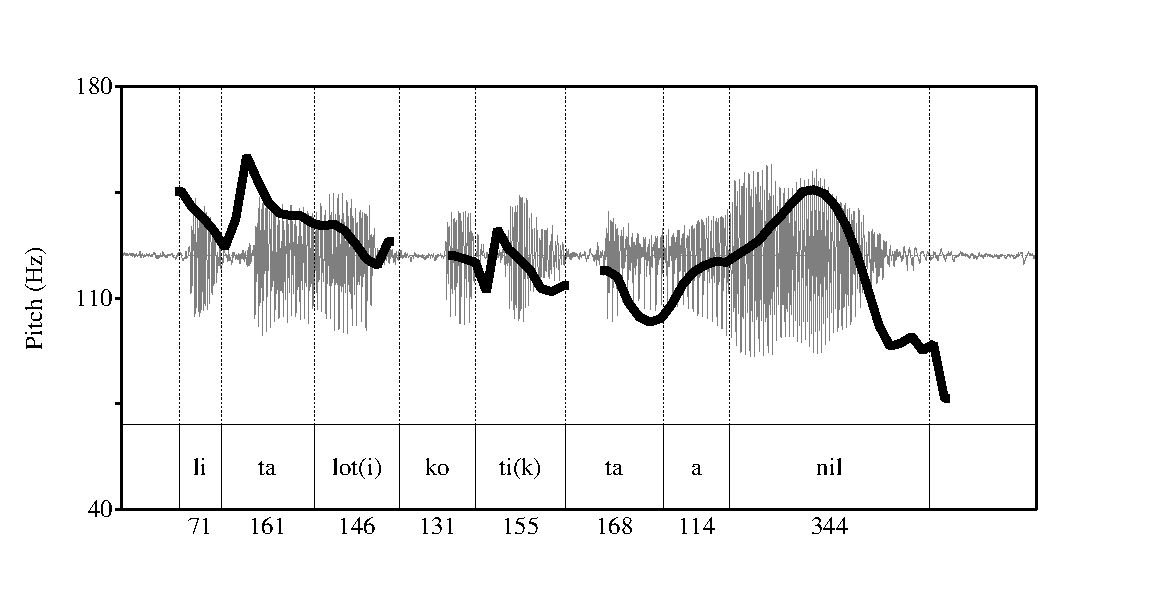
\includegraphics[width=\textwidth]{figures/aissen/anil2.eps}
\todo[inline]{figure missing}
	\caption{Pitch track and waveform for (\ref{exe:hurry}).}
	\label{fig:hurry}
\end{figure}

\begin{exe}
\ex
\gll L-i-tal-otkotik ta anil. \\
\textsc{cp-abs.1}-come-\textsc{1pl.excl} in hurry \\
\glt `We came in a hurry.'  (\textsc{author})
\label{exe:hurry}
\end{exe}

A key observation is that because =\emph{e} aligns with the right edge of the $\iota$P, then, whatever else it is, it is the 
final syllable of the $\iota$P. It thus carries the boundary tone, and is often followed by significant pause and lengthened.
This is illustrated in Figure~\ref{fig:presko}, which is based on (\ref{exe:presko}), from the same narrative as Figure~\ref{fig:hurry}; this phrase is also utterance-final.

\begin{figure}
% 	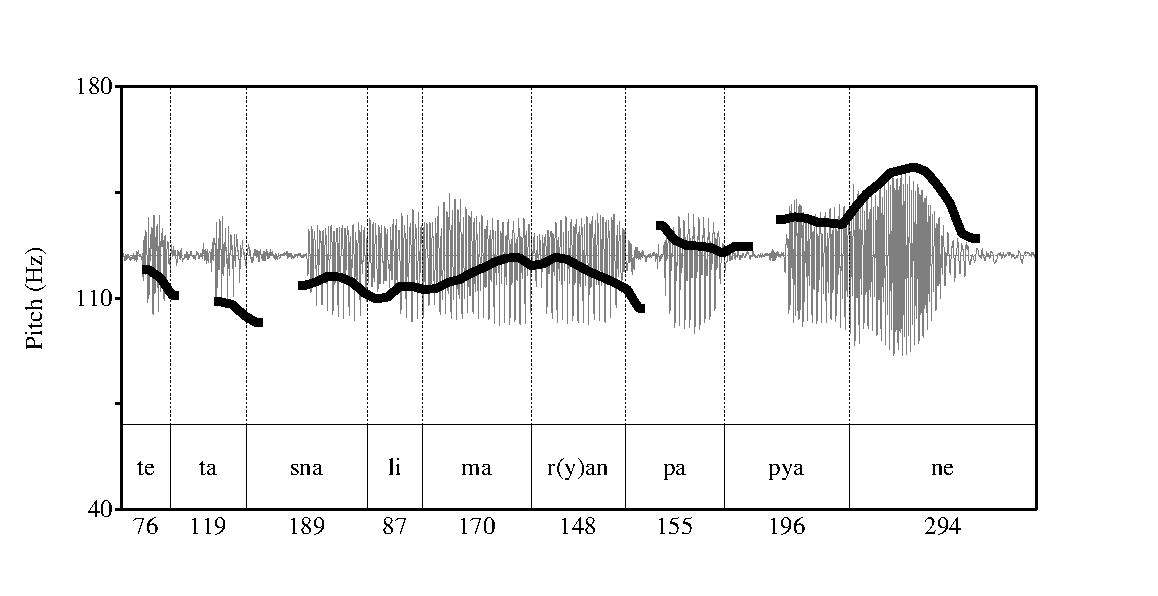
\includegraphics[width=\textwidth]{figures/aissen/papyan.eps}
\todo[inline]{figure missing}
	\caption{Pitch track and waveform for (\ref{exe:presko}).}
	\label{fig:presko}
\end{figure}

\begin{exe}
\ex\label{exe:presko}\bridgeoverex
\gll \dots {}  te ta s-na \tikzmarkfullnamed{a}{li} Maryan Papyan=\tikzmarkfullnamed{b}{e}. \\
{} there \textsc{p} \textsc{gen.3}-house \textsc{det} Mariano Papyan-\textsc{def} \\
\glt `\dots there in the house of Mariano Papyan.'  (\textsc{author})
 \bridgeover{a}{b}
 \end{exe}

The analysis proposed in \S5 hinges on the obligatory association between =\emph{e}  and the prosodic peak of $\iota$P. 

As in other languages, utterances consisting of a simple clause are parsed as a single  $\iota$P. There are also two structures in Z Tsotsil 
which  are associated with obligatory $\iota$P breaks, resulting in utterances with multiple  $\iota$P's, and therefore multiple positions 
for =\emph{e} under (\ref{exe:gen6}): an external topic is parsed as an $\iota$P separate from that of the following 
comment clause and
an extraposed \textsc{cp} is parsed as a $\iota$P separate from that the preceding matrix clause.\footnote
{Some adverbial clauses are obligatorily parsed as separate $\iota$P's and some only optionally. These are
not discussed here, but see \citet[59]{aissen1992}.}
Other complements, as well as elative clauses, are usually not extraposed and they are prosodically integrated into the $\iota$P  of the matrix clause.
In this section we provide support for (\ref{exe:gen6}), starting with simple clauses (\S3.1), then considering structures with multiple  $\iota$P's (\S3.2-\S3.3),
and finally syntactically complex structures which map to a single $\iota$P (\S3.4).  \S3.5 suggests
an algorithm for mapping syntactic structure to prosodic structure.

\subsection{Simple clauses}
In utterances consisting of a single clause, regardless of where =\emph{e} is licensed,
it appears at the right edge of the $\iota$P corresponding to the clause.
When the licensing phrase itself is clause-final, as in (\ref{exe:exe4})-(\ref{exe:lic}), that phrase has the appearance 
of being closed by =\emph{e}. 
But if a clause contains several phrases which are headed by licensors, no phrase which occurs medially can end in 
=\emph{e}. Adding it in in the positions of the asterisks in (\ref{exe:bz}) and (\ref{exe:cv}) is impossible.
		\begin{exe}
		\ex\label{exe:bz}\bridgeoverex
		\gll S-jipan la ta=ora [\tikzmarkfullnamed{a}{ti} ok'il \tikzmarkfullnamed{b}{*}] [\tikzmarkfullnamed{c}{ti} t'ul] un=\tikzmarkfullnamed{d}{e}.\\
		\textsc{erg.3}-tie \textsc{cl} right.away \textsc{det} coyote {} \textsc{det} rabbit  \textsc{par-def} \\
		\glt `The rabbit tied Coyote up right away.'  \citep[160]{laughlin1977} 
		\bridgeover{a}{b}
		\bridgeover{c}{d}
		\end{exe}
		\begin{exe}
		\ex\label{exe:cv}\bridgeoverex
		\gll I-s-ta la tal [\tikzmarkfullnamed{e}{li} aniyo \tikzmarkfullnamed{f}{*}]  ta yut=vo' [\tikzmarkfullnamed{g}{li} choy] un=\tikzmarkfullnamed{h}{e}. \\
		\textsc{cp-erg.3}-find \textsc{cl} \textsc{dir} \textsc{det} ring {}  \textsc{p} inside.water \textsc{det} fish \textsc{par-def} \\
		\glt `The fish found the ring in the water.'   \citep[354]{laughlin1977} 
		\bridgeover{e}{f}
		\bridgeover{g}{h}
		\end{exe}
One might think that =\emph{e} is simply omitted when the licensing phrase does not occur clause-finally. But examples like (\ref{exe:sob})-(\ref{exe:candle}) 
show otherwise.  Here (and generally), the clause-medial \textsc{dp} \emph{does} license =\emph{e}  but the clitic 
is delayed to the end of the clause.
%		\begin{exe}
%		\ex
%		\gll Xlichlon la jelavel [\node{i}{\underline{ti}} pepen]_{dp} [ta ti' kwartel]_{pp} un=\node{j}{\underline{e}}. \\
%		flapped \textsc{cl} by \textsc{det} butterfly \textsc{p} door prison \textsc{par-def} \\
%		\glt `Butterfly flapped by the barracks door.'  \citep[22]{laughlin1977} 
%		\barnodeconnect[.05cm]{i}{j}
%		\label{exe:ovo}
%		\end{exe}
		\begin{exe}
		\ex\label{exe:sob}\bridgeoverex
		\gll L-i-'abtej-otikotik xchi'uk [\tikzmarkfullnamed{i}{li} Kumpa Lol]\sub{dp} ta museo-\tikzmarkfullnamed{j}{e}. \\
		\textsc{cp-abs.1}-work-\textsc{1pl.excl} with \textsc{det} Compadre Lol \textsc{p} museum-\textsc{def} \\
		\glt We worked with Compadre Lol at the museum. \citep[25]{laughlin1980} 
		\bridgeover{i}{j}
		\end{exe}
		\begin{exe}
		\ex\label{exe:vov}\bridgeoverex
		\gll Ch-'och xa [\tikzmarkfullnamed{p}{\underline{li}} k'ok']\sub{dp} [ok'ob]\sub{adv} [ta Nibak]\sub{pp}=\tikzmarkfullnamed{q}{\underline{e}}. \\
		\textsc{icp}-enter \textsc{cl} \textsc{det} fire tomorrow \textsc{p} Ixtapa-\textsc{def} \\
		\glt `The war will begin tomorrow in Ixtapa.'  \citep[119]{laughlin1977} 
		\bridgeover{p}{q}
		\end{exe}
		\begin{exe}
		\ex\label{exe:candle}\bridgeoverex
		\gll Ta=x-[y]-ak'-ik [\tikzmarkfullnamed{i}{\underline{ti}} kantela]\sub{dp} [noxtok]\sub{adv}=\tikzmarkfullnamed{j}{\underline{e}}. \\
		\textsc{icp-erg.3}-give-\textsc{pl} \textsc{det} candle too-\textsc{def}. \\
		\glt `They too were offering the candles.'(\textsc{author})
		\bridgeover{i}{j}
		\end{exe}
There are two properties to note in these examples. First, =\emph{e} must be licensed by the determiner since there is no other licensor present; and second, the intervening \textsc{pp}'s and adverbs are not part of the \textsc{dp} headed by the licensor. In (\ref{exe:sob})-(\ref{exe:candle}), they modify the entire sentence (or the predicate), not the head noun. In (\ref{exe:candle}), the adverb \emph{noxtok} `too, also' is associated with additive focus on the subject `they' (= shamans in the town under discussion) not the object (`the candles')  --  the preceding discourse describes shamans from a neighboring town offering candles; the current utterance asserts that the ones in this town too were offering candles. 
  =\emph{e} attaches then outside its syntactic domain, assuming that domain to be the \textsc{dp} headed by its licensor. 
 
 Going back to (\ref{exe:bz})-(\ref{exe:cv}), the right conclusion, I think, is that both determiners require =\emph{e}, but that that 
 requirement is satisfied by the single, clause-final enclitic (see also \citealt{skopeteas2010}). 
 These cases too then involve coalescence, but in a configuration 
 different from  the one illustrated by (\ref{exe:topics}c). In (\ref{exe:topics}c), the right edges of the two \textsc{dp}'s which license
 =\emph{e} coincide, but here they do not. (\ref{exe:bz})-(\ref{exe:cv}) actually provide another kind of evidence that  =\emph{e} does not
 always close its syntactic domain: the particle \emph{un} which occurs in both examples (and in many subsequent ones) is not part of the preceding \textsc{dp}, yet
whenever it occurs, it separates =\emph{e} from its licensing phrase, (see \S5.2 on \emph{un}).

Examples like (\ref{exe:zw}) and (\ref{exe:wom}) provide further evidence that =\emph{e} can occur outside its syntactic domain: they 
show that when  the phrase that licenses =\emph{e} is preposed,  =\emph{e} still surfaces in post-verbal position, at the right edge  
of the clause. 
(\ref{exe:zw}) is from a narrative in which a mother gives advice to her son, (\ref{exe:wom}) from one about the Kennedy assassination.
		\begin{exe}
		\ex\label{exe:zw}\bridgeoverex
		\gll  [Ta sba me \tikzmarkfullnamed{w}{l}-av-ajnil]\sub{pp} ch-a-muy=\tikzmarkfullnamed{x}{e}, \\
		on top \textsc{cl} \textsc{det-gen.2}-wife \textsc{icp-abs.2}-climb-\textsc{def} \\
		\glt `It's on top of your wife that you should climb [not onto the rafters].'  \citep[56]{laughlin1977}
		\bridgeover{w}{x}
		\end{exe}	
		\begin{exe}
		\ex\label{exe:wom}\bridgeoverex
		\gll Ja' nox [\tikzmarkfullnamed{v}{li} viniketik]\sub{dp} i-laj-ik ta bala=\tikzmarkfullnamed{u}{e}. \\
		\textsc{foc} only \textsc{det} men \textsc{cp}-end-\textsc{pl} \textsc{p} bullet-\textsc{def} \\
		\glt `[The women weren't hit by the bullets], it was only the men that were wounded by bullets.'  \citep[15]{laughlin1980}
		\bridgeover{v}{u}
		\end{exe}
 In (\ref{exe:zw}), a \textsc{pp} has been fronted into focus position, as sketched 
	in (\ref{exe:sue}) (the larger context makes clear that we are dealing with corrective focus in both (\ref{exe:zw}-\ref{exe:wom})).
	Note that a fronted focus does \emph{not} occasion an $\iota$P break \citep{aissen1992}.
	\begin{exe}
		\ex\label{exe:sue} = structure of (\ref{exe:zw})\\
		\begin{forest}
			[\textsc{ip}
				[\textsc{pp}
					[ta\\\emph{\footnotesize on}]
					[nP
						[sba\\\emph{\footnotesize top}]
						[\textsc{dp}, name=DPlabel
							[{l-av-ajnil\\\emph{\footnotesize your wife}}, roof, name=DP]
						]
					]
				]
				[vP
					[{ch-a-muy=e\\\emph{\footnotesize you climb}}, roof, name=vP]
				]
			]
		\node[draw,thick,rounded corners, shape=circle, inner xsep=-20pt, inner ysep=0pt, fit=(DPlabel) (DP)] {};
		\draw[thick] ([yshift=4ex,xshift=0.5em]DP.south west) |- +(0ex,-5ex) -| ([yshift=4ex,xshift=-0.55em]vP.south east); 
		\end{forest}
	\end{exe}
\vspace*{2ex}
The  licensor for =\emph{e} in (\ref{exe:sue}) is the head of the circled \textsc{dp}, which is embedded quite deeply within the fronted \textsc{pp}, but the enclitic  does not close that \textsc{dp}. Instead it surfaces clause-finally.
 (\ref{exe:wom}) is a cleft construction where the focus occurs preverbally. Again =\emph{e} is licensed by
the head of that \textsc{dp} but occurs clause-finally (the verb phrase which follows the focus does not modify the focus and is presumably not embedded in it).

With respect then to simple, monoclausal structures, 
examples (\ref{exe:sob})-(\ref{exe:wom}) show (in various ways) that in Z Tsotsil, =\emph{e} does not in general 
close the \emph{phrase} headed by its licensor. A closer approximation is that it closes the \emph{clause} 
containing the licensor (though we will see shortly that this is not the whole story either). 
This holds whether the licensor is a determiner or some other element, e.g., a deictic adverb.  
(\ref{exe:34})-(\ref{exe:35}) show that an =\emph{e} licensed by 
a deictic adverb also occurs clause-finally, again separated from the phrase containing the licensor by intervening material (in (\ref{exe:35}),
the adverb functions as the clausal predicate).
\begin{exe}
\ex\label{exe:34}\bridgeoverex
\gll J-tsak-tik [\tikzmarkfullnamed{c}{lavi}]  [ta k'in]-\tikzmarkfullnamed{d}{e}. \\
\textsc{erg.1}-grab-\textsc{1pl.inc} today \textsc{p} fiesta \\
\glt `Let's arrest him today at the festival.' (NT: Matthew 26:5)
%\gll Ch-i-bat [\node{c}{lavi}] [noxtok] un=\node{d}{e}. \\
%\textsc{icp-abs.1}-go today again \textsc{par-def} \\
%\glt `I'm going again today.'  \citep[247]{laughlin1977}
\bridgeover{c}{d}
\end{exe}
\begin{exe}
\ex\label{exe:35}\bridgeoverex
\gll Muk'  \tikzmarkfullnamed{e}{li'} s-malal=\tikzmarkfullnamed{f}{e}. \\
\textsc{neg} here \textsc{gen}-husband-\textsc{def} \\
\glt `Their husbands weren't around here [they had gone to the lowlands].' \citep[101]{laughlin1977}
%\gll \node{e}{Li'}-on xa ox ta kriarail vo'on un-\node{f}{e}. \\
%here-\textsc{abs.1s} \textsc{cl} \textsc{cl} \textsc{p} maid \textsc{pro.1sg} \textsc{par-def} \\
%\glt `I was already  here [in San Cristobal] as a  maid.' \citep[172]{laughin1977}
%\gll Oy [\node{e}{le'}] [jun ants chamem]=\node{f}{e}. \\
%$\exists$ there \textsc{indf} woman dead-\textsc{def} \\
%\glt `There's a dead woman over there.' (lit. \dots a women who is dead). \citep[230]{laughlin1977}
\bridgeover{e}{f}
\end{exe}
\subsection{Topics}
As in many other languages, external topics in Tsotsil are parsed as separate $\iota$P's  (by `external topic', I mean one which is attached
outside the sentence, often entering into an anaphoric relation with a pronoun inside the sentence) \citep{aissen1992}.  
Topics are usually definite in Tsotsil and therefore are almost always closed by =\emph{e}
(the $\iota$P break is indicated by ``\textbardbl''):
\begin{exe}
\ex\label{exe:top4}\bridgeoverex
\gll \tikzmarkfullnamed{a}{Ti} moletik vo'ne tey ta Ats'am=\tikzmarkfullnamed{b}{e},  \textbardbl {}  i-s-tsob la s-ba-ik \\
\textsc{det} elders  long.ago there \textsc{p} Salinas-\textsc{def} {} \textsc{cp-erg.3}-gather \textsc{cl} \textsc{gen.3-rr-pl} \\
\glt {\vspace*{-3ex}}
\gll ta snuts-el  \tikzmarkfullnamed{m}{li}  biyaetik=\tikzmarkfullnamed{n}{e}.  \\
 \textsc{p} chase-\textsc{nomzl}  \textsc{det} Villistas-\textsc{def} \\
\glt `The elders of long ago (from) there in Salinas gathered to chase the Villistas.' (\textsc{author})
 \bridgeover{m}{n}
 \bridgeover{a}{b}
\end{exe}
\begin{exe}
\ex\label{exe:top3}\bridgeoverex
\gll \tikzmarkfullnamed{o}{Ti} anima j-muk'tot=\tikzmarkfullnamed{p}{e}  \textbardbl {} x-'ok' xa la sutel tal. \\
\textsc{det} late \textsc{gen.1}-grandfather-\textsc{def} {} \textsc{asp}-cry \textsc{cl} \textsc{cl} returning here \\
\glt `My late grandfather returned crying.' (\textsc{author})
 \bridgeover{o}{p}
\end{exe}

\subsection{Complex clauses with CP complements}
CP complements obligatorily extrapose in Tsotsil. While normal order in transitive clauses is \textsc{vos},
 when \textsc{o} is a \textsc{cp} complement, it occurs utterance-finally \citep{aissen1992}.
 \begin{exe}
\ex\label{exe:zzz}\bridgeoverex
\gll I-y-il  \tikzmarkfullnamed{s}{\underline{ti}} s-me' un=\tikzmarkfullnamed{t}{\underline{e}}  \textbardbl \\
\textsc{cp-erg.3}-see  \textsc{det} \textsc{gen.3}-mother  \textsc{par-def} {} \\
\glt {}
\gll ti muk'=bu ta s-sa' y-ajnil \tikzmarkfullnamed{q}{ti} s-krem un=\tikzmarkfullnamed{r}{e} . \\
\textsc{comp} \textsc{neg} \textsc{icp} \textsc{erg.3}-seek \textsc{gen.3}-wife  \textsc{det}  \textsc{gen.3}-son \textsc{par-def} \\ 
\glt `His mother saw that her son was never going to find a wife.'   \citep[55]{laughlin1977}
\bridgeover{q}{r}
\bridgeover{s}{t}
\end{exe}
Extraposition is associated with an obligatory $\iota$P break and, as expected, the matrix and \textsc{cp} complements form separate domains for clitic placement: the =\emph{e} licensed by the first determiner closes the first $\iota$P and the one licensed by the second
closes the second  $\iota$P. 

Extraposition of \textsc{cp} complements also occurs in ditransitive clauses. While the \textsc{theme} precedes the \textsc{goal} when both are nominal,
the \textsc{theme} follows the \textsc{goal} when it is a \textsc{cp}: 
\begin{exe}
\ex\label{exe:zzz2}\bridgeoverex
\gll Ikalbe \tikzmarkfullnamed{s}{li} kumpa Lol un=\tikzmarkfullnamed{t}{e}  \textbardbl {} \tikzmarkfullnamed{i}{ti} yu'un chicham xa un=\tikzmarkfullnamed{j}{e}. \\
I.told  \textsc{det} compadre Bob \textsc{par-def} {} \textsc{comp} because I.was.dying \textsc{cl} \textsc{par-def} \\ 
\glt \vspace*{-6ex}`I told Compadre Bob that I was feeling awful.' \citep[30]{laughlin1980}
\bridgeover{s}{t}
\bridgeover{i}{j}
\end{exe}
Again, extraposition forces an $\iota$P break between the matrix clause and its extraposed complement. 
And as above, the two clauses form separate domains for clitic placement. 
 
 \subsection{Prosodically integrated subordinate clauses}
While \textsc{cp} complements extrapose, there are other embedded clauses which do not and thus remain in their
base position. These include
\textsc{ip} complements (selected by verbs of perception and some other higher predicates) 
as well as relative clauses. Prosodically these do not form separate $\iota$P's, but are integrated into the $\iota$P 
of the matrix clause  (see \citealt{an2007} on languages in which restrictive relatives do not form separate $\iota$P's).

Consider the \textsc{ip} complement in (\ref{exe:ip}). It remains in its internal position and is followed by the matrix subject:
\begin{exe}
\ex\label{exe:ip}\bridgeoverex
\gll
 Mi ja'uk o=bu y-a'i [lok' \tikzmarkfullnamed{a}{ti} y-ajnil *]\sub{ip} \tikzmarkfullnamed{c}{ti} vinik un=\tikzmarkfullnamed{b}{e}. \\
 \textsc{neg} even ever \textsc{erg.3}-feel leave \textsc{def} \textsc{gen.3}-wife {} \textsc{det} man \textsc{par-def} \\
 \glt `The man didn't even feel his wife slipping out.' \citep[49]{laughlin1977}
 \bridgeoverht{3.5ex}{a}{b}
  \bridgeover{c}{b}
 \end{exe}
There is no extraposition here and the entire utterance is pronounced as a single $\iota$P. If =\emph{e} closed the (smallest) \emph{clause} in which was licensed, we would expect 
one to surface in the position of the asterisk. But =\emph{e}  is not possible there.
Instead, it appears that the enclitic licensed within the complement is delayed until the end of the entire utterance,
where it coalesces with the one licensed by the subject. Consistent with (\ref{exe:gen6}), the enclitic licensed within the complement clause is pronounced at the right edge of the $\iota$P which contains its licensor.

Relative clauses (\textsc{rc}) also generally do not extrapose. Relative clauses with external heads do not occur utterance-internally (if necessary, the sentence is restructured so that they occur utterance-finally or sentence-initially as part of the topic), but headless relatives (or better, `light-headed' relatives involving a determiner + \textsc{cp}) can.\footnote
{I take the \textsc{rc} to be a \textsc{cp} since it contains a fronted \textsc{wh} expression in (\ref{exe:rc3}) and a complementizer in (\ref{exe:rc4}).}
In (\ref{exe:rc3}) and (\ref{exe:rc4}), the \textsc{rc} is sandwiched between the matrix verb and the matrix subject. 
\begin{exe}
\ex\label{exe:rc3}\bridgeoverex
\gll Y-il-oj [ti [bu k'ot \tikzmarkfullnamed{a}{ti} j'ik'al *]\sub{RC}]  \tikzmarkfullnamed{e}{ti} vinik un=\tikzmarkfullnamed{b}{e}. \\
\textsc{erg.3}-see-\textsc{prf} \textsc{det} where arrive \textsc{det} Spook {} \textsc{det} man \textsc{par-def} \\
\glt `The man saw (the place) where the Spook landed.' \citep[63]{laughlin1977}
 \bridgeoverht{3.5ex}{a}{b}
 \bridgeover{e}{b}
\end{exe}
\begin{exe}
\ex\label{exe:rc4}\bridgeoverex
\gll I-y-a'i la [taj [k'alal ch-lok' tal \tikzmarkfullnamed{c}{taj} \\
\textsc{cp-erg.3}-feel \textsc{cl} \textsc{det} when \textsc{icp}-leave \textsc{dir} \textsc{det} \\
\glt {\bridgeoverex}
\gll {\phantom{\hspace*{1in}}} chon *]\sub{RC}] \tikzmarkfullnamed{f}{taj} ants un=\tikzmarkfullnamed{d}{e}, \\
{} serpent  {}  \textsc{det} woman \textsc{par-def} \\
\glt `That woman felt (the moment) when that snake left.'  \citep[371]{laughlin1977}
 \bridgeover{c}{d}
 \bridgeover{f}{d}
\end{exe}
Like \textsc{ip} complements, \textsc{rc}'s do not constitute separate $\iota$P's, but are parsed together with the matrix clause.  
Examples (\ref{exe:rc3})-(\ref{exe:rc4}) show that an =\emph{e} licensed in such a relative clause is realized not at the edge of the relative clause (marked here by an asterisk), but again at the right edge of the entire utterance where it coalesces with the clitic licensed by the matrix subject.

\subsection{Summary}
The position in which =\emph{e} is pronounced in Z Tsotsil does not coincide with the edge of the phrase in which is licensed, nor even 
with the edge of the (minimal) clause in which it is licensed. Rather, it  coincides with the right edge of $\iota$P containing
its licensor.  

While it is not necessary for our purposes to provide an algorithm for mapping syntactic structure to
prosodic structure (what is important is that  $\iota$P breaks fall in certain positions, not why they fall there), there is a simple
principle which determines this mapping if we assume that external topics and extraposed clauses are both adjoined at the root
of the sentence \citep{aissen1992}.
 Assuming that an element X which adjoins to Y is not dominated by Y, then neither topics nor extraposed clauses are dominated by any node. Hence, like simple clauses, the nodes which define these consituents are `undominated'. In this respect they are like root nodes
 and, following \citet{frank2002ais}, I will refer to them as such.
With this understanding, the mapping from syntax to $\iota$P can be characterized as a \emph{match} between a certain syntactic constituent (one dominated by a root node) 
and a corresponding prosodic constituent (an $\iota$P) (on \textsc{Match} constraints, see \citealt{selkirk2009} and \citealt{elfner2012};  on the relevance of the \emph{root} to defining $\iota$P, see \citealt{downing1970, nesporvogel1986, selkirk2009}). The formulation in (\ref{exe:match}) is based on \citet{bennettetal} and \citet{elfner2012},
\begin{exe}
\ex
\textsc{Match Root} \\
If a root node \emph{R} in a syntactic representation \emph{S} dominates all and only the set of terminal elements \{\emph{a,b,c, \dots, n}\}, 
then there must be in the phonological representation \emph{P} corresponding to \emph{S} an $\iota$P which dominates all and only
 the phonological exponents of \emph{a,b,c, \dots, n}.
\label{exe:match}
\end{exe}
When \textsc{Match Root} is satisfied in Tsotsil (as it appears always to be), 
simple clauses and some complex structures are parsed as single $\iota$P's; extraposed CP's and topics are  parsed into their own $\iota$P's.  

In \S5, I develop an account of clitic placement in Tsotsil in which the syntax positions =\emph{e} at the edge of the phrase in which
it is licensed, per (\ref{exe:defp}), and the phonology accounts for its subsequent dislocation to the right edge of $\iota$P.  This attributes
a more significant role to the phonology than some theories of clitic placement permit.
Hence before turning to the phonological account,
I consider the prospects for accounts in which phonology plays at most a filtering role in the placement of =\emph{e} in Tsotsil.

\section{A syntactic account?}
While recognizing that the positioning of some clitics is sensitive to prosodic constituency, some recent theories of
clitic placement propose that the role of phonology is limited to filtering outputs from the syntax. 
Consider, for example, \citet{boskovic2000}'s account of 
second-position clitics in Serbo-Croatian.
Bo\v{s}kovi\'{c} argues that these clitics attach to the first prosodic word within an $\iota$P. 
This is a prosodic generalization, but in his account, the prosody does not directly determine the position of second-position clitics. 
Rather, clitics reach their surface positions through syntactic mechanisms.
Since syntactic mechanisms sometimes place clitics in other than `second' position, PF filters out derivations 
in which the clitics do not suffix to the initial prosodic constituent in the $\iota$P. 
\citet{otero2011} propose that all cases of prosodic conditioning of clitic placement can be handled in the same way,
i.e., clitics are positioned by a possibly over-generating syntax, with ill-formed configurations filtered out at PF.

The problem posed by =\emph{e} is clear.   If its syntactic domain is the phrase headed by its licensor (typically, \textsc{dp}), 
then the syntax should place =\emph{e} somewhere within that domain.
However, we have seen that =\emph{e} can occur outside the phrase in which it is licensed, indeed outside the  
clause in which it is licensed. In fact, it \emph{must} occur outside that phrase (or clause) when it is not $\iota$P-final.
The only option for  an account of clitic placement in which phonology does no more than filter outputs from the syntax is to extend
 the syntactic domain of =\emph{e} (or the [+\textsc{def}] feature which it realizes) beyond  the 
phrase in which it is licensed. 
 
Conceived syntactically, the dependency between the position in which =\emph{e} is licensed and the position in 
which it is pronounced can span a significant amount of syntactic structure  --  it crosses clause-boundaries including ones
which define relative clauses. There are various ways that apparent long-distance dependencies are handled, depending
both on the nature of the dependency and on the particular syntactic model  -- 
long-distance movement (Transformational Grammar), a sequence of local movements (Minimalism), 
feature percolation (GPSG/HPSG) and others \citep{alexiadou2012a}. 
It is beyond the scope of this article to develop a syntactic analysis of =\emph{e} placement, but we can point out
two properties of the phenomenon that any such analysis must account for. 
One is that the top of the dependency is limited to root (undominated)
nodes: =\emph{e} can spell out only at the right edge of an undominated node, and not at the right edge of any other node. 
If movement or percolation are involved, they must therefore be to the root, whether that node corresponds to a simple clause,
a topic, or an extraposed complement. The other is that the bottom of the dependency can be located \emph{anywhere} 
within the structure dominated by the root. In particular, it can  be located within a constituent which is otherwise an island for extraction,
for example within a \textsc{pp}, as in (\ref{exe:zw}/\ref{exe:sue}) (see \citealt{aissen1996} for evidence that \textsc{pp}'s 
are islands for extraction), or a relative clause, (\ref{exe:rc3})\--(\ref{exe:rc4}) (see \citealt{aissen1992}). 

It is instructive to consider a particular analysis which would position =\emph{e} in its low, syntactically-licensed position 
and account  for its appearance at the right edge of $\iota$P's through late, prosodically-conditioned linearization.
  \citet{otero2011} mention this as a possible analysis for cases in which a clitic attaches to a 
 prosodically defined domain, like the second position clitics in Chamorro \citep{chung2003}. 
 They point to Linear Syntax \citep{kathol2004}, a theory of linearization embedded in
HPSG, as a possible framework for implementation. Linear Syntax imposes precedence relations on sisters but, in order to handle 
discontinuities, permits those relations to be `passed up' the tree and then `shuffled' with relations among higher elements. In this way, 
elements from an embedded domain may be separated from one another by elements that belong to higher syntactic domains.
In the case at hand, =\emph{e}, linearized, for example at the right edge of
the phrase in which it is licensed, could be separated from that phrase at higher levels, extending its syntactic domain to a higher 
consituent. 

The question for this account is just what constraints it imposes on the upward `percolation' of 
precedence relations. In a language which does not in general permit scrambling, which nodes pass precedence relations upwards and which do not?
The most obvious challenge is posed by the fact that an =\emph{e} licensed somewhere within a relative clause or a \textsc{pp} cannot surface
within those phrases if they are not utterance-final, but must surface in the matrix.  
In the shuffling account of examples like (\ref{exe:zw}/\ref{exe:sue}) and (\ref{exe:rc3})-(\ref{exe:rc4}),
 the precedence relation between =\emph{e} and the rest of the licensing phrase (its specifier, under (\ref{exe:defp})) would be obligatorily
passed up through the relative clause or \textsc{pp} and then shuffled with precedence relations among elements  in the matrix clause. 
Since \textsc{pp}'s and relative clauses are otherwise impermeable in Tsotsil, one must 
 wonder why Shuffling, but not other syntactic operations, can access elements within them. 
 
 On the other hand, it is a prosodic fact, independent of anything about =\emph{e}, that \textsc{pp}'s and relative clauses in 
 Tsotsil do not form separate $\iota$P's. Hence the fact that  an =\emph{e} licensed within them surfaces outside them when they
 are not utterance-final follows from the prosodic generalization in (\ref{exe:gen6}).  
 In short, if the relation between =\emph{e} and the phrase in which it is licensed is conceived as a syntactic dependency, 
 its properties are unexpected. 
But if the relation is instead phonological and holds 
 within an $\iota$P at a point when syntactic structure is no longer relevant, the distribution of =\emph{e} and
its relation to the licensing phrase begin to make sense.

\section{A prosodic account}
\subsection{Association with prosodic prominence}
I outline here an account of  =\emph{e} in Z Tsotsil. This account shares with Anderson's \citeyear{anderson2005} approach to clitic placement the assumption that the surface position
 of =\emph{e} is determined post-syntactically through an optimization that evaluates alternative positions of the clitic against a set of ranked constraints  \citep{prince1993}. 
  It differs from Anderson in that  =\emph{e} is not itself subject to a constraint which aligns it with the edge of a constituent. Rather the position of =\emph{e} is motivated by an 
inherent lexical property, namely its association with the prosodic prominence that characterizes the right edge of $\iota$P's in the language.
 In this, I closely follow  \cite{henderson2012ais}'s account of certain `status' suffixes in K'iche' (also Mayan),\footnote 
{These suffixes mark the transitivity status of the predicate and make other distinctions related to mood and dependency.} 
which surface only at the right edge of $\iota$P. These suffixes attach only to verbs
and surface only when the verb occurs $\iota$P-finally, (\ref{exe:kiche}a). Otherwise, the suffix is suppressed, (\ref{exe:kiche}b)  (accent marks here represent the prosodic
peak of the utterance):
\begin{exe}
\ex
\begin{xlist}
\exi{a.}
\gll X-in-\underline{tij-\'o}. \\
\textsc{cp-erg.1sg}-eat-\textsc{ss} \\
\glt `I ate it.'
\exi{b.}
\gll X-in-\underline{tij} le s\'ub'. \\
\textsc{cp-erg.1sg}-eat \textsc{det} tamalito \\
\glt `I ate the tamalito.' \citep[775--776]{henderson2012ais}
\end{xlist}
\label{exe:kiche}
\end{exe}
Henderson notes that status suffixes are simply omitted from phrase-medial verbs, rather than being displaced to $\iota$P-final position
(see \ref{exe:kiche}b) and attributes this to the fact that the suffix is an affix (not a clitic) and attaches only to verbs.
 He raises the issue of what would happen if the element in question were a clitic. 
The distribution of Tsotsil =\emph{e} instantiates exactly this case: =\emph{e} is not tied to any particular
word class and thus faithful realization carries it away from the position in which it is licensed.

The lexical entry for =\emph{e} is shown in (\ref{exe:lex}), where the asterisk indicates association with
the prosodic peak of $\iota$P:
\begin{exe}
	\ex\label{exe:lex}
	\begin{forest}
		[$\ast$
			[\emph{e}]
		]
	\end{forest}
\end{exe}
I also adopt Henderson's constraint set, it being as well-suited to Tsotsil =\emph{e} as it is to the K'iche' status suffixes. 
The constraints fall into three groups. 
The first two concern the location of prosodic prominence in the $\iota$P and are independent
of the distribution of =\emph{e}. 
An alignment constraint \citep{mccarthy1993}
 locates the peak of prosodic prominence at the right edge of the $\iota$P, (\ref{exe:c1}).
\textsc{Culminativity} (\ref{exe:c2}) limits such peaks to one per $\iota$P \citep{hayes1995}.
\begin{exe}
\ex \textsc{Align$_{\iota}$}:  A peak of prominence lies at the right edge of the $\iota$P.
\label{exe:c1}
\end{exe}
\begin{exe}
\ex \textsc{Culm(inativity)}: Every prosodic domain has exactly one peak of prominence.
\label{exe:c2}
\end{exe}
The second two are faithfulness constraints on the morphology-to-phonology correspondence \citep{prince1993,mccarthy1995}.
 \textsc{RealizeMorph} (\ref{exe:c3}), a general
constraint, calls for faithful parsing of morphemes in the phonology \citep{kurisu2001}. 
\textsc{IdentProm} (\ref{exe:c4}) is the key constraint here: it requires that the lexical association of =\emph{e} with prosodic prominence be preserved in the output \citep{henderson2012ais}.\footnote
{I have slightly reworded \textsc{IdentProm} from Henderson to emphasize the distinction between M in the input
and its correspondent M' in the output.} 
\begin{exe}
\ex \textsc{RealizeM(orph)}: Every morpheme in the input has a phonological exponent in the output.
\label{exe:c3}
\end{exe}
\begin{exe}
\ex \textsc{IdentProm}: if morpheme M has prominence P in the input, then M', the phonological correspondent of M, 
has prominence P in the output.
\label{exe:c4}
\end{exe}
Tableau~(\ref{exe:tableau1}) shows the effect of these constraints on the evaluation of an input, that of (\ref{exe:sob}), in which the syntactically determined
position for =\emph{e} does not correspond to the right edge of an $\iota$P. 
The input in Tableau~(\ref{exe:tableau1}) is a morphophonological representation in which syntactic terminals 
have been spelled-out and in which the hierarchical structure of syntax has been replaced by precedence relations and 
prosodic structure. =\emph{e} is a morphophonological element. Its position is syntactically determined per 
(\ref{exe:defp}) and its association with the prosodic peak is indicated in the input by the asterisk, a morphological diacritic.
Candidates for the output are fully linearized phonological representations, parsed into prosodic constituents. 
 Prosodic prominence in the $\iota$P is marked by an acute accent.  
\begin{exe}
	\ex\label{exe:tableau1}Tableau for (\ref{exe:sob})\\
	\footnotesize
	\begin{tabular}[t]{|l@{\hspace{2pt}}r@{\hspace{2pt}}l||c:c:c:c|}%{|l@{\hspace{2pt}}r@{\hspace{2pt}}l| | c :c  : c : c |}	
		\hline	
		\multicolumn{3}{|l||}{\multirow{2}{*}{\let\eachwordone=\footnotesize\let\eachwordtwo=\footnotesize\gll [\dots{} li Kumpa Lol=e* ta museo]$_{\iota}$ \\
		\dots{} \textsc{det} compadre L-\textsc{def} \textsc{p} museum \\}}  & \multirow{2}{*}{\textsc{Align$_{\iota}$}}   &\multirow{2}{*}{\textsc{Culm}}   & \textsc{Ident}  &   \textsc{Realize}  \\ 	
		& & & & & \textsc{Prom} & \textsc{Morph} \\
		\midrule %\hline
		a. & &  [\dots li kumpa lol=\'e ta museo]$_{\iota}$  &$\ast$!   &               			& &                              	 \\
		\midrule		
		b. & \hand & [\dots li kumpa lol ta museo=\'e]$_{\iota}$ &	&               		& &		                    	 \\
		\midrule
		c. & & [\dots li kumpa lol=e ta muse\'o]$_{\iota}$		&                  	&  &		$\ast$! &		        \\ 
		\midrule
		d. & &  [\dots li kumpa lol-\'e ta muse\'o]$_{\iota}$		&                     	&	$\ast$!	  & &		        \\ 
		\midrule
		e. & &   [\dots li kumpa lol ta museo]$_{\iota}$		&                     	& &		 &		$\ast$!        \\
		\hline
	\end{tabular}
\end{exe}
 \noindent
The optimal candidate is [b], which violates none of the constraints shown. However, it does violate one which is not shown, 
\textsc{Linearity}, which penalizes outputs which diverge from the precedence relations of the input \citep{mccarthy1995}.\footnote
{The high-ranked constraint \textsc{Match Root} (\ref{exe:match}) prevents =\emph{e} from moving `too far', by requiring that it be realized 
within the same $\iota$P as its licensor.
\label{footnote:matchroot}
}
\textsc{Linearity}
must be lower ranked than any of the four constraints shown in Tableau~(\ref{exe:tableau1}).
\begin{exe}
\ex \textsc{Lin(earity)}: The precedence structure of the input is consistent with that of the output and vice versa.
\label{exe:c5}
\end{exe}

When the input has two enclitics, they coalesce in the output. 
\begin{exe}
		\ex\label{exe:bz2}\bridgeoverex
		\gll S-jipan la ta=ora [\tikzmarkfullnamed{a}{ti} ok'il [\tikzmarkfullnamed{c}{ti} t'ul] un=\tikzmarkfullnamed{d}{e}.\\
		\textsc{erg.3}-tie \textsc{cl} right.away \textsc{det} coyote \textsc{det} rabbit  \textsc{par-def} \\
		\glt `The rabbit tied Coyote up right away.'  \citep[160]{laughlin1977} 
		\bridgeoverht{3.5ex}{a}{d}
		\bridgeover{c}{d}
		\end{exe}
Taking the input to (\ref{exe:bz2}) to be [\dots ti ok'il=e* ti t'ul=e*], we can see that the optimal output,  [b] in Tableau 2, 
violates none of the four constraints (\ref{exe:c1})-(\ref{exe:c4}): the prosodic peak is aligned with the right edge of the $\iota$P, 
there is only a single prosodic peak, the prosodic prominence associated with =\emph{e} in the input is preserved in the output, and 
every morpheme in the input has a phonological exponent in the output. The association of input morphemes to phonological 
exponents, however, is many-to-one, as indicated by the subscripts on =\emph{e} in input and output.
Hence the optimal candidate, [b] (=\ref{exe:bz2}), violates the Anti-Coalescence constraint, \textsc{Uniformity} \citep{mccarthy1995}, 
as well as \textsc{Linearity}.
Like \textsc{Linearity}, \textsc{Uniformity} is ranked below the other constraints shown.
\begin{exe}
\ex \textsc{Unif(ormity)}: No element in the output has multiple correspondents in the input.
\label{exe:c6}
\end{exe}

\begin{exe}
	\ex\label{exe:tableau2}Tableau for (\ref{exe:bz2})\\
	\footnotesize
	\begin{tabular}[t]{|l@{\hspace{2pt}}r@{\hspace{2pt}}l@{}||c:c:c:c|c:c|}	
		\hline
\multicolumn{3}{|@{\hspace{2pt}}l@{}||}{\multirow{2}{*}{\let\eachwordone=\footnotesize\let\eachwordtwo=\footnotesize\gll [\dots ti ok'il=e*\sub{1} ti t'ul=e*\sub{2}]$_{\iota}$ \\
\dots \textsc{det} coyote-\textsc{def} \textsc{det} rabbit-\textsc{def}\\}} & \multirow{2}{*}{\textsc{Align$_{\iota}$}}   & \multirow{2}{*}{\textsc{Culm}}   & \textsc{Ident}  &   \textsc{Realize} & \multirow{2}{*}{\textsc{Lin}} & \multirow{2}{*}{\textsc{Unif}} \\ 	
& & & & & \textsc{Prom} & \textsc{Morph} & & \\
%& \rot{\textsc{Align$_{\iota}$}}  & \rot{\textsc{Culm}}  &  \rot{\textsc{IdentProm}} &  \rot{\textsc{RealizeM}} & \rot{\textsc{Lin}} & \rot{\textsc{Unif}} \\
\hline \hline
a. && [\dots ti ok'il=\'e\sub{1} ti t'ul=\'e\sub{2}]$_{\iota}$ 	&  $\ast$ &            $\ast$ 			& 	&                 & &      	 \\
\hline		
b. & \hand & [\dots ti ok'il ti t'ul=\'e\sub{1,2}]$_{\iota}$       &	      &               		&           &		 &$\ast$ &             $\ast$                 \\
\hline
c. & & [\dots ti ok'il ti t'ul=\'e\sub{2}]$_{\iota}$       &	      &               		&           &		$\ast$  & &                             \\
\hline		
d. & & [\dots ti ok'il=e\sub{1} ti t'ul=\'e\sub{2}]$_{\iota}$       &	      &               		&      $\ast$    &		 & &                            \\
\hline
e. & &  [\dots ti ok'il=\'e\sub{1,2} ti t'ul]$_{\iota}$		&   $\ast$                	& &		 &	    & $\ast$ & $\ast$   \\ 
\hline	
f. & &   [\dots ti ok'il ti t'ul]$_{\iota}$		&                     	& &	 &		$\ast$$\ast$   & &  \\ 
\hline	
g. & &   [\dots ti ok'il ti t'ul=\'e\sub{1}=\'e\sub{2}]$_{\iota}$		&                     	& $\ast$ &		 &		 & $\ast$ &    \\ 
\hline
 \end{tabular}
\end{exe}
\noindent
Candidates not shown include variations on [g] in which one =\emph{e} or the other does not realize the prosodic prominence of the
$\iota$P, i.e., [\dots \emph{ti t'ul=e\sub{1}-\'e\sub{2}}] and [\dots \emph{ti t'ul-\'e\sub{1}=e\sub{2}}]. Both violate \textsc{IdentProm} and the second one violates \textsc{Align}$_{\iota}$ as well.

Some additional facts, not yet presented, show that \textsc{RealizeMorph} must be indexed for particular morphemes and that
the one which indexes =\emph{e} is ranked below \textsc{Align$_{\iota}$}, \textsc{Culminativity} and  \textsc{IdentProm}.
The definite enclitic  =\emph{e} is
not the only morpheme in Zinacantec Tsotsil which is lexically associated with the prosodic peak of $\iota$P. 
The other is an epistemic particle, \emph{a'a}, which \citet{laughlin1975}
classifies as an `exclamation' and translates  \emph{indeed!, surely! certainly! of course!}. \emph{a'a} does not require licensing, though statistically, it tends to occur in utterances with 1st and/or 2nd person arguments and is likely cognate
with a reduplicated form of the terminal clitic \emph{a'} \textsc{`proximate'} in Yucatec.  
Relevant here is that \emph{a'a} occurs in the same position as =\emph{e}, i.e., at the right edge of
$\iota$P, with its second syllable functioning as the prosodic peak of $\iota$P. 
\begin{exe}
\ex
\begin{xlist}
\exi{a.}
\gll Ta'ajebal \underline{li} j-ve'el-tik a'a. \\
almost.cooked \textsc{det} \textsc{gen.1}-meal-\textsc{1pl.inc} \textsc{exclam} \\
\glt `Our meal certainly is about cooked.' \citep[285]{laughlin1977}
\exi{b.} 
\gll Ta j-ti' \underline{lavi}  a'a.\\
\textsc{icp} \textsc{erg.1}-eat today \textsc{exclam}   \\
\glt  `Of course I'll eat it today.' \citep[283]{laughlin1977}
\exi{c.}
\gll Ik'-o \underline{le'} a'a! \\
take-\textsc{imp} \textsc{dem} \textsc{exclam} \\
\glt `Take her!' \citep[126]{laughlin1977}
\exi{d.}
\gll  A li Pineda=e mas mas ts'akal a'a. \\
\textsc{top} \textsc{det} Pineda-\textsc{def} more more afterwards  \textsc{exclam} \\
\glt `Pineda was later, of course.' \citep[116]{laughlin1977} 
\end{xlist}
\label{exe:a'a}
\end{exe}
=\emph{e} and \emph{a'a} compete
with one another, with priority given to realization of \emph{a'a}. Thus =\emph{e} must be omitted when \emph{a'a} occurs. 
 (\ref{exe:a'a}a-c) contain various elements
(underlined) that otherwise require =\emph{e} (see Table~\ref{table:licensors}). Here though, \emph{a'a} entirely precludes realization of =\emph{e}.

As an epistemic operator, I assume that \emph{a'a} occupies a position in the syntax; its
exact locatiion cannot be determined  since it is pronounced only at the right edge of $\iota$P. 
 Assuming that \emph{e*} and \emph{a'a*} can both be present in the input,
 one or the other must `disappear'. Which is preserved is determined by the ranking of morpheme-specific \textsc{RealizeM} constraints. In  Zinacantec Tsotsil, \textsc{Realize}(a'a*) $\gg$ \textsc{Realize}(=e*). The overall ranking of the constraints under discussion then is shown in Figure~\ref{fig:ranking}.
\begin{figure}
	\begin{tikzpicture}[text height=1.5ex, text depth=0.25ex]
 	\node(Align) at (-4,0) {\textsc{Align}$_{\iota}$} ;
 	\node(Culm) at (-1.5,0) {\textsc{Culminativity}};
 	\node(Ident) at (1.5,0) {\textsc{IdentProm}};
 	\node(RMa) at (4,0) {\textsc{Realize}(\emph{a'a*})};
 	\node(RMe) at (0,-1.5) {\textsc{Realize}(=\emph{e*})};
 	\node(Lin) at (-2,-3) {\textsc{Linearity}};
 	\node(Unif) at (2,-3) {\textsc{Uniformity}};
 	\draw (Align.south) -- (RMe.north);
 	\draw (Culm.south) -- (RMe.north);
 	\draw (Ident.south) -- (RMe.north);
 	\draw (RMa.south) -- (RMe.north);
 	\draw (RMe.south) -- (Lin.north);
 	\draw (RMe.south) -- (Unif.north);
 	\end{tikzpicture}
    \caption{Constraint ranking}
    \label{fig:ranking}
    \end{figure}
    
  \subsection{Notes on the right periphery}
I close this section by discussing the relation between the terminal elements =\emph{e} and \emph{a'a}, and two other elements which `pile up' at the right periphery. The ordering of the four is shown in (\ref{exe:periphery}):
\begin{exe}
\ex 
\begin{tabular}[t]{| c | c | c |}
\hline
 \emph{un} & =\emph{e/a'a} & \emph{che'e} \\
 \hline
\textsc{par} & \textsc{def/exclam} & \emph{`then'} \\
 \hline
 \end{tabular}
 \label{exe:periphery}
 \end{exe}
The particle \emph{un} occurs in many of the examples cited above. 
No meaning (propositional or otherwise) has yet been identified for it. Some speakers have the intuition
that it contributes some nuance of meaning to the sentence; others say that the sentence just `sounds better' with it. 
\emph{un} has a distribution similar to that of =\emph{e} and \emph{a'a}: like them, \emph{un} occurs at 
the right periphery of root sentences and of topics, and it can separate a matrix clause from its extraposed complement.
Also like them, it occurs in no other positions. Unlike =\emph{e}, it is not lexically licensed.

 \citet{aissen1992} analyzed \emph{un} as an enclitic which aligns with the right edge of $\iota$P. 
While it is true that \emph{un} always occurs very near the right edge of $\iota$P,  it does not occur rightmost when any of the other elements in (\ref{exe:periphery}) is present. 
While it is not yet clear what is responsible for its appearance and position, I assume that it is not lexically associated
with the prosodic peak in $\iota$P and that its position is therefore not determined by \textsc{IdentProm}. For one thing, as
observed in \citet{skopeteas2010}, it does not coalesce with =\emph{e} (nor with \emph{a'a}). 
One possibility is that it is present already at Spell-Out at the right edge of $\iota$P. 
It would then be present in the \emph{input} to evaluations like those in Tableaux 1 and 2,
 and the constraint ranking in Figure~\ref{fig:ranking} would position \emph{e} and \emph{a'a} to its right.
Another possibility is that \emph{un} is introduced by the phonology for eurhythmic reasons, e.g., 
to improve the prosodic structure of the utterance, perhaps at lower levels of the prosodic hierarchy. 
I leave further  development of these ideas for a later time.

The other element in (\ref{exe:periphery}) is \emph{che'e}, which occurs only in the absolute final position.  
\emph{che'e} is a discourse particle which \citet{laughlin1975} translates
as `then' (roughly Spanish \emph{pu\'es}): 
\begin{exe}
\ex\label{exe:che'ee}\bridgeoverex
\gll L-i-bat xa \tikzmarkfullnamed{e}{li} vo'on=\tikzmarkfullnamed{f}{e} che'e, \\
\textsc{cp-abs.1}-go \textsc{cl}  \textsc{det} \textsc{pro.1sg}-\textsc{def} then \\
\glt `Me, I went, then.'  \citep[131]{laughlin1977}
\bridgeover{e}{f}
\end{exe}
\emph{che'e} can cooccur with =\emph{e} and when
it does, the high boundary tone appears to be realized on the last syllable of \emph{che'e}, 
not on =\emph{e}. It seems then to be a counterexample to the descriptive
generalization that =\emph{e} is always the prosodic peak of the $\iota$P in which it occurs.   

A plausible scenario is that \emph{che'e} is incorporated into the $\iota$P which ends in =\emph{e} after the point
at which the constraints discussed above have had an effect.
Fleshing this out a little, \emph{che'e} might be syntactically adjoined to the root and mapped into its own $\iota$P (like topics and
extraposed clauses). This $\iota$P being however subminimal (two syllables, one word), \emph{che'e} is incorporated into the preceding $\iota$P
(on the tendency to avoid short $\iota$P's or sequences of $\iota$P's of different length, see \citealt{nesporvogel1986} and \citealt{dehe2009}).
 The result here is to push =\emph{e} back from the edge, and for the boundary tone to fall on the final syllable of \emph{che'e}.  
 An account along these lines assumes
 that the constraints in Figure~\ref{fig:ranking} apply within the domain of  $\iota$P's that result from the initial 
 prosodic parsing and do not reapply at a later stage when prosodic restructuring of multiple $\iota$P's occurs.
 If they did, =\emph{e} would be reordered again, to the right of \emph{che'e}. How such an account with
 its implied serial optimization fits into the larger theory of the syntax-phonology interface remains to be seen.

\section{An historical scenario}
Definite markers which close the phrase in which they are licensed are not uncommon \citep{wals-37}.\footnote
{Languages with such markers include Wolof (Niger-Congo,  \citealt{torrence2013}), Basque \citep{laka1996}, Angami (Tibeto-Burman, \citealt{Giridhar-1980}, cited in \citealt{wals-37}), and Gaahmg (Nilo-Saharan, \citealt{stirtz2012}).
} 
  It is plausible then that the definite enclitic =\emph{e} in Z Tsotsil might, at an earlier stage, have been the final element in the noun
  phrase, a position in which it would not necessarily have functioned as the prosodic peak of $\iota$P.
  Here I offer a suggestion for how =\emph{e} might have come to be associated with that peak, an association
  which now sometimes forces it out of its licensing phrase.
 
The basic idea is simple:  the syntax usually determines an utterance-final position 
for the \emph{phrase which licenses =\emph{e}}. Hence even without intervention from the phonology,  
=\emph{e} would have found itself in most cases at the right edge of the utterance.
As such, it would become statistically associated with the prosodic peak of the $\iota$P 
 and this could have been reanalyzed as a lexical property.  

There are several reasons why the syntax usually puts the \emph{phrase} which licenses
=\emph{e} in utterance-final position. A number of them come down to the fact that certain grammatical relations in
Tsotsil are almost always instantiated by definite noun phrases and the syntax determines a position for
these relations at the right edge of the utterance anyway.  
These include especially subjects, possessors, and topics. The usual ordering of these elements is shown in (\ref{exe:wordorder}).
Starting with topics, as we have already seen, the topic precedes its associated clause and always constitutes its own $\iota$P.
As the final element in the topic then, =\emph{e} automatically falls at the right edge of $\iota$P.   
\begin{exe}
\ex
\begin{itemize}
\item[\textopenbullet]
Topic  X
\item[\textopenbullet]
V\--O\--S
\item[\textopenbullet]
Possessum \-- Possessor
\end{itemize}
\label{exe:wordorder}
\end{exe}
Basic word order in Tsotsil is usually described as VOS, with the subject in clause-final position. Transitive subjects (as well as active
intransitive ones) are almost always definite, so generally license =\emph{e}. Unless the subject is followed by some other element (e.g.,
an adverb, a PP, an element in a matrix clause), =\emph{e} again finds itself at the right edge of $\iota$P.
Finally, Tsotsil being a head-initial language, the possessor follows its possessum, as in (\ref{exe:juan}).
 \begin{exe}
 \ex\label{exe:juan}\bridgeoverex
 \gll L-i-bat ta [s-na [\tikzmarkfullnamed{e}{li} Xun=\tikzmarkfullnamed{f}{e}]]. \\
 \textsc{cp-abs.1}-go \textsc{p} \textsc{gen.3}-house \textsc{det} Juan-\textsc{def} \\
 \glt `I went to Juan's house.'
  \bridgeover{e}{f}
 \end{exe} 
 Possessors too are almost always definite, and often end up as the final phrase in an utterance. Here too,
 =\emph{e}'s position at the right edge of $\iota$P is determined by the syntax. In all these cases then,
 =\emph{e} is the last syllable in $\iota$P, the position associated with the prosodic peak. 
  
 Of course, the phrase which licenses =\emph{e} does not always occur utterance-finally -- if it did, there would be no
 motivation for this paper.  But in a fragment of written text containing 156 instances of =\emph{e}, there were only three in which
 that phrase did \emph{not} occur utterance-finally. In these cases, 
  =\emph{e} was separated from its licensing phrase, as in  (\ref{exe:sob})-(\ref{exe:sue}) above. Thus, if it is true that
 the position of =\emph{e} was originally determined syntactically, it would nonetheless have had a
 statistical association with the phonological properties that characterize the prosodic peak of $\iota$P and
reanalysis of this association as a lexical property would have resulted in the situation we see today.  

\section{Conclusion}
This paper has attempted to lay out the case for Z Tsotsil =\emph{e} as a special clitic  --  
one whose surface position is not always a position it could have reached syntactically. If this is correct, the phonology does something here \emph{other} than select the prosodically optimal position for =\emph{e} from among the syntactically possible ones. It must achieve the effect of moving =\emph{e} within a prosodically-defined domain. In the analysis proposed here, =\emph{e} is not subject to an alignment constraint; rather, it ends up at the right edge of $\iota$P because it must function as the prosodic peak of $\iota$P, and that peak is located at the right edge of $\iota$P. Complying with this requirement sometimes involves reordering the enclitic over a fairly large distance. Since the reordering occurs in the phonology, it is not subject to syntactic locality. It is, though, subject to prosodic locality, as =\emph{e} always remains within the $\iota$P  that contains its licensor 
(fn.~\ref{footnote:matchroot}). 

Tsotsil =\emph{e} thus appears to be different from the the second position clitics discussed in \citet{boskovic2000} and \citet{otero2011}, clitics which can reach their surface positions by syntactic means. The difference might be understood in terms of the property which determines their surface position. The position of the second-position clitics of Chamorro and Serbo-Croatian is determined by a prosodic alignment condition. But prosodic constituency is introduced in the interface between syntax and phonology and is therefore present before the phonology proper.  The placement of second-position clitics can therefore be determined prior to the phonology and without any involvement of the phonology.  On the other hand, if the analysis of Z Tsotsil =\emph{e} suggested here is on the right track, its position  cannot be determined until the phonology proper, since it is only in the phonology that the location of prosodic prominence within the $\iota$P is fixed at the right edge. In this light, the special clitic status of =\emph{e} arises because the condition which makes it `special'  --  which forces it out of its licensing phrase  --  references a purely phonological property and not a prosodic edge.  \\

\section*{Abbreviations}
\begin{multicols}{2}
\noindent
\textsc{asp}:  aspect\\
\textsc{cl}: clitic\\
  \textsc{cp}: completive aspect\\
        \textsc{def}: definite terminal clitic\\
   \textsc{dir}: directional \\
   $\exists$: existential predicate \\
    \textsc{exclam}: exclamatory particle \\
  \textsc{icp}: incompletive aspect\\
    \textsc{p}: preposition\\
    \textsc{pro}: pronoun \\
        \textsc{par}: particle \\
      \textsc{rr}: reflexive/reciprocal \\
      \textsc{ss}: status suffix \\
          \end{multicols}


\section*{Acknowledgements}
Earlier versions of this paper were presented at UCSC, UC Berkeley, and at \emph{Exploring the interfaces III}, McGill U. 
I would like to thank all those who have given me feedback on this material, especially a number of anonymous reviewers  -- 
their comments were extremely helpful. I owe special thanks to Ryan Bennett, both for his comments on an earlier version and for
 sustained discussion of various issues relevant to this material. Ryan also prepared the pitch tracks included here. Needless to say
 I alone am responsible for the content of the paper.
 
I am delighted to contribute a paper on clitics to a festschrift which honors Steve Anderson. Steve's work in this area, as in others, has been
foundational. But on a more personal note, it was at his suggestion in 1972 that I went to Mexico for the first time to work on Tsotsil. 
Steve was thus directly responsible for the direction my career took and I am glad to be able to thank him for that here.


\printbibliography[heading=subbibliography,notkeyword=this]
% \todos

\end{document}
